\documentclass[12pt]{article}
\usepackage[russian]{babel}
\usepackage[utf8]{inputenc}
\usepackage{graphicx}
\usepackage{amsmath}
\usepackage{float}
\usepackage{geometry}
\usepackage{longtable}
\usepackage{enumitem}
\usepackage{listings}
\usepackage{xcolor}
\usepackage{indentfirst} % Для отступов в первом абзаце
\usepackage{subcaption} 
\usepackage[skip=5pt]{caption}
\usepackage{siunitx}
\usepackage{booktabs}
\usepackage{array}
\usepackage{hyperref}
\usepackage{setspace}

% Настройки русской типографии
\geometry{a4paper, left=30mm, right=15mm, top=20mm, bottom=20mm}
\setlength{\parindent}{1.25cm} % Красная строка
\setlength{\parskip}{0pt}      % Убираем отступы между абзацами
\linespread{1}               % Полуторный интервал

% Настройка гиперссылок
\hypersetup{
    colorlinks=true,
    linkcolor=blue,
    urlcolor=blue,
    citecolor=black,
}

% Стиль библиографии
\bibliographystyle{gost2015}

% Настройка листингов
\lstdefinelanguage{JavaScript}{
    keywords={let, const, function, return},
    sensitive=false,
    morecomment=[l]{//},
    morecomment=[s]{/*}{*/}
}

\lstset{
    basicstyle=\ttfamily\small,
    keywordstyle=\color{blue},
    commentstyle=\color{green},
    stringstyle=\color{red},
    numbers=left,
    numberstyle=\tiny\color{gray},
    frame=single,
    breaklines=true
}

% Настройка формата чисел
\sisetup{
    output-decimal-marker = {.},
    group-digits = false
}

\begin{document}

\tableofcontents

\newpage

\section{Введение}

В современном мире скорость загрузки веб-сайта играет критически важную роль для обеспечения положительного пользовательского опыта (User Experience, UX)
и достижения высоких позиций в результатах поиска. С увеличением требований пользователей к быстродействию и доступности информации оптимизация
скорости разгрузки сайтов стала неотъемлемой частью процесса разработки веб-приложений.
Медленная загрузка страниц может привести к ухудшению показателей вовлеченности, увеличению показателя отказов и, как следствие,
снижению рейтинга сайта в поисковых системах.

Одним из способов увеличения скорости загрузки является применение сжатия для статических файлов, изображений и запросов. При этом необходимо грамотно подбирать степень сжатия
из-за накладных расходов на компрессию и декопрессию. Мы попытаемся определить \textbf{оптимальные} с определённой точки зрения параметры сжатия в зависимости от характеристик
аппаратной части клиента и сервера, пропускной способности сети.

Также сжатие позволяет снизить нагрузку на сеть и существенно сэкономить трафик. Может показаться,
что в современном мире высокоскросного интернета на это уже не стоит обращать внимание.
Но на весну 2025 года, Amazon (\url{https://aws.amazon.com/ru/cloudwatch/pricing/}) требует 0,5\text{\$} за 1ГБ трафика. Что для небольших IT стартапов является существенной строкой расхода.

На просторах интернета существует уже достаточно много сравнений популярных методов сжатия, таких как Gzip и Brotli, Jpeg и WebP:

\begin{itemize}
    \item Brotli и GZIP: \href{https://medium.com/@bansal.suneet/brotli-vs-gzip-compression-surprising-compression-result-brotli-power-782aac2ee29f}{Meduium Brotli и GZIP}
    \item Brotli и GZIP: \href{https://ddos-guard.ru/blog/algoritmy-brotli-recompressiya-i-HSTS-chto-novogo-predlagaet-DDoS-GUARD}{DDoS-Guard о Brotli}
    \item Jpeg и WebP: \href{https://medium.com/@inna_netum/действительно-ли-webp-лучше-jpeg-91639d852035}{Сравнение WebP и JPEG}
\end{itemize}

Но в основном в своих работах авторы ограничиваются такими параметрами как степень сжатия, скорость компрессии/декомпрессии,
что тяжело переложить на ключевые метрики, такие как LCP (Largest Contentful Paint, время до отрисовки самого большого элемента) и RPS (Requests Per Second, число запросов в секунду).

Основная задача - определить и обосновать оптимальные параметры сжатия для загрузки и работы Web-приложений в условиях изменяющейся сетевой нагрузки.
В рамках работы предполагается разработка системы, способной адаптировать параметры сжатия в реальном времени для обеспечения бесперебойного
функционирования и быстрого отклика приложений, учитывая изменение числа пользователей и интенсивности их активности.

\section{Описание объекта исследования}

В ходе данной работы мы будем тестировать алгоритмы сжатия на примере REST AP
(Representational State Transfer Application Programming Interface / Программный интерфейс приложения для передачи репрезентативного состояния)
SPA (Single page application / Одностраничное веб-приложение) веб-приложения, выполняющего роль видеохостинга.
Сжатие видео в ходе данной работы не рассматривается

Видеохостинг должен выполнять следующую бизнес-логику:

\begin{itemize}
    \item Аутентифицировать пользователей
    \item Возможность добавлять, удалять, просматривать видео
    \item Подбирать персональные рекомендации
    \item Оставлять комментарии и ставить лайки под видео
\end{itemize}

\subsection{Стек технологий}

\begin{figure}[H]
    \centering
    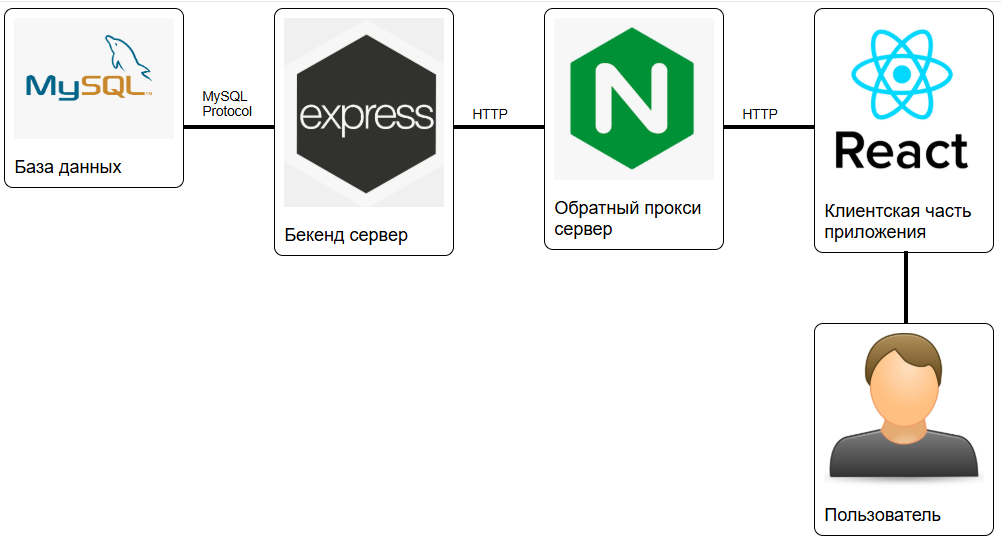
\includegraphics[width=1\textwidth]{../images/Схема_веб-приложения.png}
    \caption{Схема веб приложения}
\end{figure}

Вкратце опишем для чего нужен каждый элемент схемы:

\begin{itemize}
    \item \textbf{Backend} сервер обрабатывает запросы от пользователя, отвечает за аутентификацию,
          реализует бизнес логику. Например: подобрать рекомендации видео для конкретного пользователя, загружать/удалять видео
    \item \textbf{Frontend} - это часть веб-приложения, что находится на стороне пользователя.
          Пользователь загружает статические файлы сайта, которые в последующем исполняются в браузере.
          HTML отвечает за разметку, CSS добавляет стили, а JS отвечает за функциональность - делает сайт живым
    \item \textbf{База данных} необходима для удобного хранения большого количества данных
    \item \textbf{Обратный прокси сервер} выполняет вспомогательные операции с запросами.
          Помимо перенаправления запросов, он также может выполнять сжатие, кеширование, предоставлять доступ к файлам,
          балансировать нагрузку
\end{itemize}

Используется следующий стек технологий:

\begin{itemize}
    \item Express JS - backend сервер
    \item React JS - frontend часть приложения
    \item MySQL - реляционная база данных
    \item Nginx - обратный прокси сервер
\end{itemize}

\subsection{Характеристики аппаратной части сервера}

\begin{itemize}
    \item CPU 1 vCPU
    \item RAM 2 GB
    \item Storage 20 GB
    \item Speed 500 Mbps
\end{itemize}

\subsection{Сценарий работы пользователя}

Пользователь переходит по ссылке или вводит в строку поиска http://example-videohosting.ru.
В этом случае на сервер передаётся HTTP Get запрос, по которому находится \verb|index.html| файл.

Этот файл выглядит следующим образом:

\begin{lstlisting}[language=HTML]
<!DOCTYPE html>
<html lang="en">
<head>
    <meta charset="UTF-8">
    <meta name="viewport" content="width=device-width, initial-scale=1.0">
    <title>Videohosting</title>
    <link rel="stylesheet" href="./main.css">
    <script src="./main.js"></script>
</head>
<body>
    <img src="./assets/images/image.png">
    ...
</body>
</html>
\end{lstlisting}

После загрузки файла браузер начинает его обрабатывать:

\begin{itemize}
    \item Cтроится DOM (Document Object Model / представление HTML-документа в виде дерева элементов)
    \item Подгружаются CSS файлы (строка 7)
    \item Подгружаются и исполняются JS файлы (строка 8)
    \item Подгружаются и отрисовываются изображения (строка 11)
\end{itemize}

Когда этот процесс завершится, можно считать, что приложение полностью загружено и готово к использованию.

Далее пользователь может выполнять HTTP запросы для отправки форм, скачивания данных с backend сервера.

Исходя из вышесказанного, мы можем применять сжатие для \textbf{статических данных} (файлов сайта)
и \textbf{динамических данных}. Дадим более подробное определение введённых понятий:

\begin{itemize}
    \item Статические данные - это данные, которые неизменны для каждого пользователя. К ним можно отнести HTML, JS, CSS файлы сайта и в целом все изображения
    \item Динамические данные - это данные, меняющиеся во время работы приложения.
          К ним можно отнести информацию о видео (видео могут добавляться/удаляться, изменяется количество просмотров, отметок нравится и т.д)
\end{itemize}

Мы отдельно рассмотрим сжатие статических и динамических данных.

Начнём с рассмотрения методов сжатия изображений

\subsection{О форматах изображений}

Перед тем как приступить к описанию форматов приведу критерии, по которым я буду их сравнивать:

\begin{itemize}
    \item \textbf{Степень сжатия} - отношение размеров исходного (формат PNG) и сжатого изображений
    \item \textbf{Скорость компрессии/декомпрессии} - как быстро сервер сожмёт изображение и как быстро клиент его разархивирует и отрисует
    \item \textbf{Совместимость с разными браузерами} - важный параметр,
          так как формат с низким процентом совместимости не может использоваться в реальном приложении
          из-за риска потерять большую часть пользователей. Для оценки этого параметра
          я буду использовать данные с сайта https://caniuse.com/, являющимся де-факто авторитетным справочником
          о технологиях в браузере.
\end{itemize}

\subsubsection{JPEG}

Filename extension: jpg jpeg jpe jif jfif jfi \\
MIME type: image/jpeg

JPEG (Joint Photographic Expert Group) поддерживается всеми браузерами,
один из самых популярных форматов изображений. \\
Поддерживаются изображения с линейным размером не более 65535 x 65536 пикселов. \\

Алгоритм JPEG наиболее эффективен для сжатия фотографий, содержащих реалистичные сцены
с плавными переходами яркости и цвета. Для хранения чертежей, текстовой и знаковой
графики лучше использовать PNG, GIF,
либо использовать режим сжатия Lossless JPG.

Уделим этому формату больше внимания чем остальным, так как он зарекомендовал себя временем
и применяется много больше других. Позволяет сжимать изображения как с потерями,
так и без потерь.
На примере JPEG, мы также постараемся понять, как можно регулировать степень сжатия.

При сжатии изображение преобразуется из цветового пространства $RGB$ в $YC_{b}C_{r}$.
Стандарт ISO/IEC 10918-1 не регламентирует в    бор именно YCbCr,
допуская другие виды преобразования.

$Y$ - компонента яркости, $С_{B}$, $C_{R}$ - синяя и красная цветоразностные компоненты

Пространство $YC_{b}C_{r}$  выбрано не случайно. Связано это с тем, что глаз намного лучше различает
яркость, нежели цветовые оттенки для которых выполняется прореживание, где каждому блоку
из 4 пикселей (2x2) ставится в соответствие усреднённое значение $C_{B}$, $C_{R}$ (Схема прореживания 4:2:0).
При этом для каждого блока 2x2 вместо 12 значений (4$Y$, 4$C_{B}$, 4$C_{R}$)
ставится в соответствие 6 значений (4$Y$, $C_{B}$, $C_{R}$). Если к изображению предъявляются более высокие
требования по качеству, могут применяться схемы по сжатия (4:4:0), (4:2:2)
или не применятся вовсе. (4:4:4)

Стандарт допускает прореживание блоков не 2*2, а 4*1 или 1\*4,
но на практике такие схемы применяются довольно редко.

После этого компоненты $Y$, $C_{B}$, $C_{R}$ разбивается на блоки 8*8.
Каждый такой блок подвергается дискретному косинусному преобразованию (ДКП)

Формула для вычисления коэффициентов ДКП $F(u,v)$ блока 8×8:

Коэффициенты ДКП $F(u,v)$ вычисляются по формуле:

\[
    F(u,v) = \frac{C(u)C(v)}{4} \sum_{x=0}^{7} \sum_{y=0}^{7} f(x,y) \cdot \cos\left(\frac{(2x+1)u\pi}{16}\right) \cos\left(\frac{(2y+1)v\pi}{16}\right)
\]

где:
\begin{itemize}
    \item $f(x,y)$ — значение пикселя в позиции $(x,y)$,
    \item $u,v$ — частотные координаты (от 0 до 7),
    \item $C(k)$ — нормировочный коэффициент:
          $
              C(k) = \begin{cases}
                  \frac{1}{\sqrt{2}} & \text{при } k=0, \\
                  1                  & \text{иначе}.
              \end{cases}
          $
\end{itemize}

Далее к полученной матрице применяется квантование (зависит от степени сжатия):

\[
    Q(u, v) = round(\frac{F(u, v)}{Q_{table}(u, v)})
\]

После этого многие высокочастотные коэффициенты становятся нулевыми.

Далее полученные коэффициенты записываются в массив и кодируются с помощью кодов Хаффмана, о которых
будет рассказано в разделе '2.4 О алгоритмах сжатия данных без потерь'

\subsubsection{PNG}

Filename extension: png\\
MIME type: image/png

PNG (Portable Network Graphics) — это растровый формат изображения, который предлагает сжатие
без потерь. Еще одна особенность PNG формата — поддержка альфа-канала (прозрачности).

Согласно сайту caniuse.com поддерживается 92,6\% браузеров весной 2025 года.

\subsubsection{Webp}
Filename extension: webp\\
MIME type: image/webp

WebP — это формат изображений, разработанный Google, который предлагает сжатие изображений
с потерями и без потерь. Он призван обеспечить высокое качество изображений при меньших размерах файлов.\\

Согласно сайту caniuse.com поддерживается 95,92\% браузеров весной 2025 года.

\subsubsection{AVIF}

AVIF (AV1 Image File Format) — это современный формат изображений,
основанный на технологии сжатия AV1. Он предназначен для обеспечения высокого
качества изображений при более низком размере файлов. Согласно сайту caniuse.com
поддерживается 92,6\% браузеров.

Согласно сайту caniuse.com поддерживается 93,71\% браузеров весной 2025 года.

\subsubsection{HEIF/HEIC}

Filename extension: heif heic\\
MIME type: image/heif image/heic\\

HEIF (High Efficiency Image Format) — это современный формат изображений,
который обеспечивает высокую эффективность сжатия и поддержку различных функций,
таких как анимация, HDR, прозрачность и многослойность.

HEIC (High Efficiency Image Container) — это контейнерный формат файла,
который используется в том числе и для хранения изображений в формате HEIF,
как пример можно привести Live Photos сделанные на iPhone.

Согласно сайту caniuse.com поддерживается 13,99\% браузеров весной 2025 года,
только устройствами Apple. По причине низкой совместимости в измерениях участвовать не будет.

\subsubsection{SVG}

Filename extension: svg\\
MIME type: image/svg+xml

SVG (Scalable Vector Graphics) — это формат изображений, основанный на XML,
который описывает двумерные векторные графики с использованием векторных объектов,
таких как линии, кривые, формы и текст. Используется для логотипов и векторных изображений.
Для растровых изображений не подходит, поэтому в измерениях участвовать не будет.

Согласно сайту caniuse.com поддерживается 96,99\% браузеров весной 2025 года.

\subsection{Об алгоритмах сжатия данных без потерь}

\subsubsection{Алгоритм Хаффмана}

\textbf{Префиксный код} - такой код, ни один символ которого не входит в любой другой.

Идея алгоритма состоит в том, что если мы знаем вероятности появления символов,
можно описать процедуру построения оптимальных префиксных кодов. Оптимальность
означает, что $H <= L H + 1$, где $L$ - средняя длина кода на символ, $H$ - энтропия.
Символам с наибольшей вероятностью ставятся в соответствии более короткие коды.

Алгоритм на входе получает таблицу частотностей символов в сообщении.
Далее на основании этой таблицы строится дерево кодирования Хаффмана.

На данный момент, браузером поддерживаются два основных алгоритма метода сжатия без потерь, применяемых для текстовых файлов (css, html, js):

\begin{itemize}
    \item Gzip
    \item Brotli
\end{itemize}

Перед тем как приступить к описанию приведённых алгоритмов, следует рассказать
о семействе алгоритмов LZ, в частности LZ77, так как оба алгоритма основываются на нём.
Алгоритмы словарного сжатия Зива-Лемпела появились во второй половине 70-х гг.
Это были так называемые алгоритмы LZ77 и LZ78, разработанные совместно
Зивом (Ziv) и Лемпелом (Lempel). В дальнейшем первоначальные схемы подвергались множественным
изменениям, в результате чего мы сегодня имеем десятки достаточно самостоятельных алгоритмов
и бессчетное количество модификаций.

LZ77 и LZ78 являются универсальными алгоритмами сжатия,
в которых словарь формируется на основании уже обработанной части входного потока,
т. е. адаптивно. Принципиальным отличием является лишь способ формирования фраз.

\subsubsection{Алгоритм LZ77}

Алгоритм LZ77 является родоначальником целого семейства словарных схем - так называемых
алгоритмов со скользящим словарем, или скользящим окном. Действительно,
в LZ77 в качестве словаря используется блок уже закодированной последовательности.
Как правило, по мере выполнения обработки положение этого блока относительно начала
последовательности постоянно меняется, словарь "скользит" по входному потоку данных.
Скользящее окно имеет длину N, т. е. в него помещается N символов, и состоит из двух
частей:

\begin{itemize}
    \item последовательности длины W=N-n уже закодированных символов, которая и является словарем
    \item упреждающего буфера, или буфера предварительного просмотра,
          длины n; обычно n на порядки меньше W.
\end{itemize}

Пусть к текущему моменту времени мы уже закодировали $t$ символов, последние $W$ символом будут
составлять наш словарь. На каждой итерации алгоритма мы ищем самое длинное вхождение префиксной
строки упреждающего буфера, начиная с $t+1$ символа в словаре + упреждающем буфере,
но важно, чтобы часть строки лежала в словаре. Полученная в результате поиска фраза
кодируется с помощью двух чисел:

\begin{enumerate}
    \item Смещения (offset) от начала буфера
    \item Длины соответствия, или совпадения
          Смещение и длина соответствия играют роль указателя (ссылки),
          однозначно определяющего фразу.
          Дополнительно в выходной поток записывается символ $s$,
          непосредственно следующий за совпавшей строкой буфера.

\end{enumerate}

Что касается декодирования сжатых данных, то оно осуществляется путем простой
замены кода на блок символов, состоящий из фразы словаря и явно передаваемого символа.
Естественно, декодер должен выполнять Те же действия по изменению окна,
что и кодер. Фраза словаря элементарно определяется по смещению и длине,
поэтому важным свойством LZ77 и прочих алгоритмов со скользящим окном является очень
быстрая работа декодера.

Алгоритмы со скользящим окном характеризуются сильной несимметричностью по времени - кодирование значительно медленнее декодирования,
поскольку при сжатии много времени тратится на поиск фраз.

\subsubsection{Алгоритм LZ77}

\subsubsection{Формат Deflate}

Формат словарного сжатия Deflate, предложенный Кацем (Katz),
используется популярным архиватором GZIP.
Сжатие осуществляется с помощью алгоритма типа LZH, иначе говоря,
указатели и литералы кодируются по методу Хаффмана.
Формат специфицирует только работу декодера, т. е. определяет алгоритм декодирования,
и не налагает серьезных ограничений на реализацию кодера. В принципе в качестве алгоритма сжатия может применяться любой работающий со скользящим окном, лишь бы он исходил из стандартной процедуры обновления словаря для алгоритмов семейства LZ77 и использовал задаваемые форматом типы кодов Хаффмана
Закодированные в соответствии с форматом Deflate данные представляют собой набор блоков,
порядок которых совпадает с последовательностью соответствующих блоков исходных данных.
Используется 3 типа блоков закодированных данных:

\begin{enumerate}
    \item Состоящие из несжатых данных;
    \item Использующие фиксированные коды Хаффмана;
    \item Использующие динамические коды Хаффмана.
\end{enumerate}

Длина блоков первого типа не может превышать 64 Кб, относительно других ограничений по размеру нет. Каждый блок типа 2 и 3 состоит из двух частей:

\begin{itemize}[label=-]
    \item описания двух таблиц кодов Хаффмана, использованных для кодирования данных блока;
    \item собственно закодированных данных.
\end{itemize}

Коды Хаффмана каждого блока не зависят от использованных в предыдущих блоках.
Cамо описание динамически создаваемых кодов Хаффмана является, в свою очередь,
также сжатым с помощью фиксированных кодов Хаффмана, таблица которых задается форматом.

Алгоритм словарного сжатия может использовать в качестве словаря часть предыдущего блока
(блоков), но величина смещения не может быть больше 32 Кб.

Данные в компактном представлении состоят из кодов элементов двух типов:

\begin{itemize}[label=-]
    \item литералов (одиночных символов);
    \item указателей имеющихся в словаре фраз; указатели состоят из пары
          <длина совпадения, смещение>
\end{itemize}

Длина совпавшей строки не может превышать 258 байт, а смещение фразы - 32 Кб.
Литералы и длины совпадения кодируются с помощью одной таблицы кодов Хаффмана,
а для смещений используется другая таблица; иначе говоря,
литералы и длины совпадения образуют один алфавит.
Именно эти таблицы кодов и передаются в начале блока третьего типа.

\subsubsection{Формат сжатия Gzip (GNU zip)}

Это утилита для сжатия и распаковки файлов, которая широко используется в UNIX-системах.
Формат файла gzip состоит из 3 основных частей:

\begin{enumerate}
    \item Заголовок: Содержит информацию о типе файла, имени оригинального файла, времени создания, уровне сжатия и других параметрах.
    \item Тело: Содержит сжатые данные, выполненные с помощью алгоритма DEFLATE.
    \item Контрольная сумма (CRC-32) и Размер оригинала: Эти данные предоставляют возможность проверки целостности и правильности распаковки данных.
\end{enumerate}

Заголовок файла содержит следующие ключевые поля:

\begin{itemize}[label=-]
    \item ID1 и ID2: Идентификаторы, указывающие на формат gzip (значения - 0x1F и 0x8B).
    \item CM: Метод сжатия (в gzip используется значение 8 для DEFLATE). \*
    \item FLG: Биты флагов, которые указывают наличие дополнительных полей и информации.
    \item MTIME: Время последней модификации оригинального файла.
    \item XFL: Дополнительная информация о методе компрессии.
    \item OS: Платформа, на которой был создан/сжат файл (gzip).
\end{itemize}

Другие значения для этого поля теоретически могут быть использованы для обозначения
различных методов сжатия, но сам формат gzip и его стандартная реализация подразумевают
использование только DEFLATE. На практике, если gzip файл содержит метод сжатия,
отличный от DEFLATE, стандартные утилиты для работы с gzip файлами могут его не поддерживать
и не распознать.

\subsubsection{За счёт чего можно добиться разных степеней сжатия?}

Т.к формат Deflate не имеет четкой спецификации алгоритма словарного сжатия,
разработчики могут использовать различные модификации LZH, подбирая параметры для
обеспечения желаемого соотношения скорости и коэффициента сжатия.
Как вариант, можно ограничить длину совпадающей последовательности

\subsection{Инструменты разработчика браузера}

\subsubsection{Браузеры и JavaScript}

На сегодняшний день существует два вида браузеров:

\begin{itemize}[label=-]
    \item Основанные на движке Chromium V8 от Google (https://github.com/v8/v8) такие,
          как Gooogle Chrome, Yandex Browser, Microsoft Edge и другие
    \item Firefox, использующий Quantum
\end{itemize}

Дело в том, что JavaScript, использующийся в веб приложениях,
- скриптовый язык, существует спецификация ESMA Script https://262.ecma-international.org/,
в которой написано, что должен делать язык, но реализация не указана.
Реализация функций языка ложится на разработчиков браузеров.
Здесь, в отличие от Си или Java, не существует компиляторов или Java Virtual Machine.
Разработчики веб-приложений точно не знают, что происходит "под капотом".

Для получения информации о времени выполнения, скорости загрузки,
использования памяти можно использовать инструменты разработчика (DevTools).
Её можно открыть в любом браузере, нажав F12

\subsubsection{Какие функции предоставляет консоль разработчика}

Реализации DevTools отличаются в зависимости от браузера.
Но в целом, DevTools у браузеров на Chromium очень похожи.
Я буду брать примеры из Google Chrome

Нас интересуют две вкладки:

\subsubsection{Networks}

\begin{figure}[H]
    \centering
    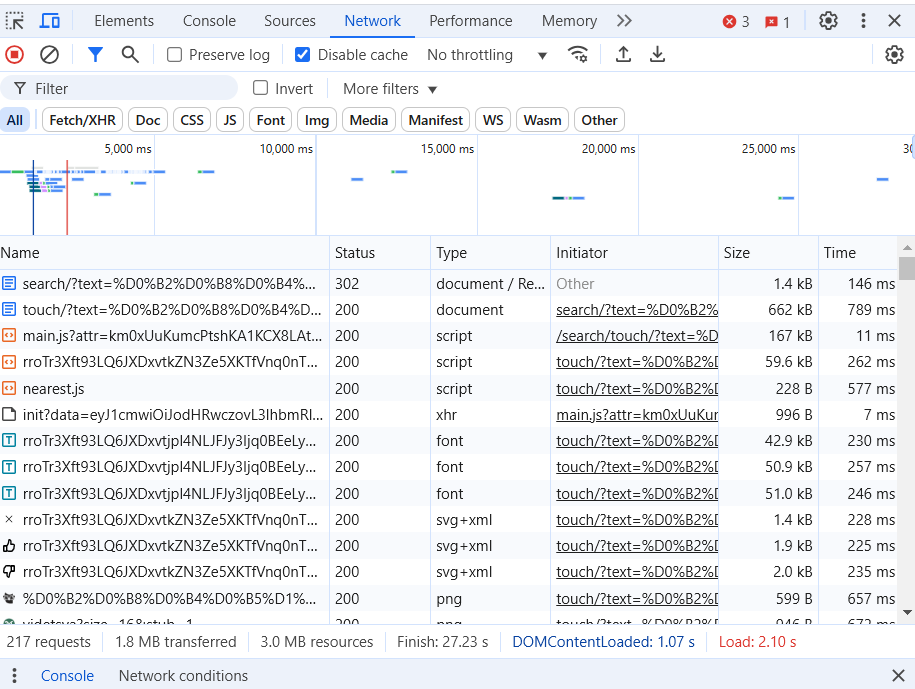
\includegraphics[width=1\textwidth]{../images/network.png}
    \caption{Вкладка Network}
\end{figure}

На этой вкладке можно посмотреть все сетевые запросы, выполненные браузером на данной странице,
узнать статус запроса, тип, размер ответа и общее время, потраченное на HTTP запрос

Если нажать на конкретный запрос, можно будет узнать такие временные интервалы, как

\begin{itemize}[label=-]
    \item Время, когда запрос был отправлен (время отсчитывается от момента перехода на сайт)
    \item Queueing Очередь . Браузер ставит запросы в очередь перед началом соединения и когда:
          Есть запросы с более высоким приоритетом. Приоритет запроса определяется такими факторами, как тип ресурса, а также его расположение в документе.
          Для этого источника уже открыто шесть TCP-соединений, что является пределом. (Применимо только к HTTP/1.0 и HTTP/1.1.)
          Браузер ненадолго выделяет место в дисковом кеше.
    \item Stalled Запрос мог быть остановлен после начала соединения по любой из причин, описанных в Queueing
    \item Initial connection. Временные затраты на TSL/SSL handshake, если используется HTTPs, на TCP Handshake
    \item Время, затраченное, на отправку запроса
    \item Время ожидание ответа от сервера
    \item Сколько времени затрачено на загрузку содержимого запроса
\end{itemize}

\begin{figure}[H]
    \centering
    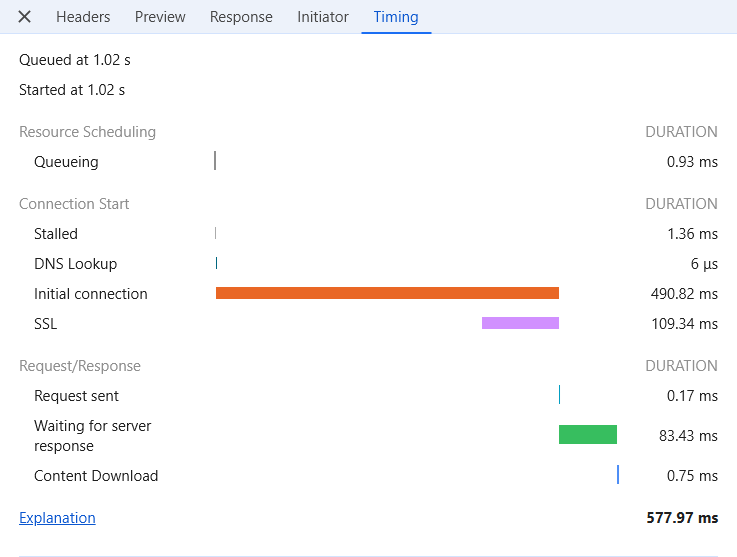
\includegraphics[width=1\textwidth]{../images/network__timing.png}
    \caption{Временные интервалы конкретного запроса}
\end{figure}

Суммарное время запроса складывается из всех перечисленных отрезков времени
Как можно заметить, по этим параметрам не удаётся определить время,
затраченное на декодирование запроса

\textbf{Немного о HTTP}

Считаю уместным сказать несколько слов о HTTP протоколе, чтобы иметь лучшее представление,
о том, как с технической точки зрения применяется сжатие.
Первым делом браузер осуществляет HTTP запрос, прикрепляя заголовок \textbf{Accept-encoding}.
Современные браузеры поддерживают Gzip, Deflate, Brotli, Zstandard,
и заголовок выглядит следующим
образом: \textbf{Accept-encoding: gzip, deflate, br, zstd}.
Сервер обрабатывает запрос, применяя к телу HTTP запроса один из алгоритмов,
указанных в \textbf{Accept-encoding}. В ответе сервер прикрепляет заголовок \textbf{Content-encoding},
например \textbf{Сontent-encoding: br}, говорящий о применённом алгоритме. Браузер получив ответ,
может продолжить загрузку тела HTTP запроса.

\subsubsection{Performance}

\begin{figure}[H]
    \centering
    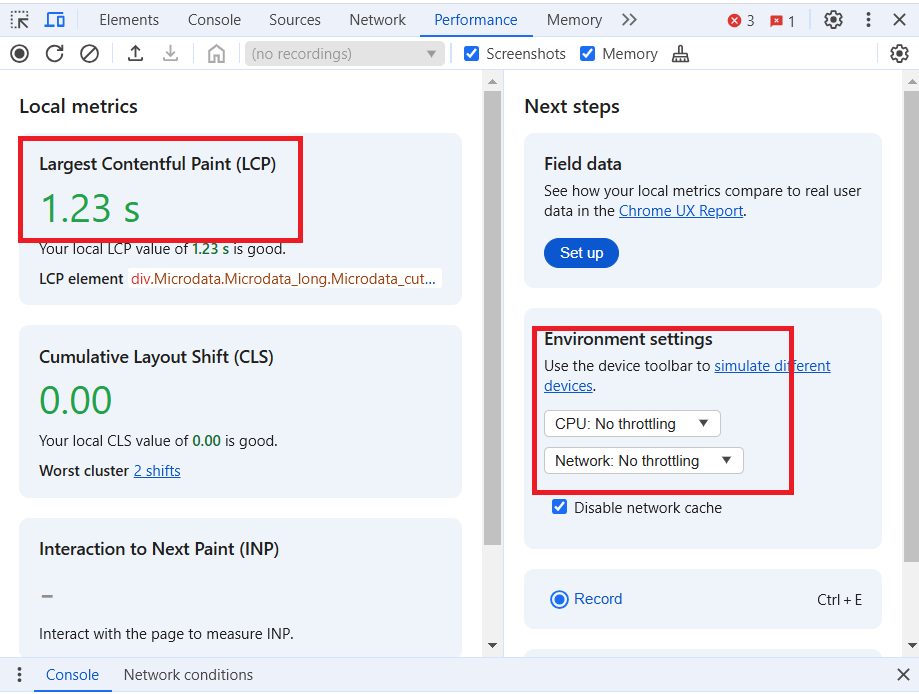
\includegraphics[width=1\textwidth]{../images/performance.png}
    \caption{Performance}
\end{figure}

На этой вкладке мы так же можем применить замедление к процессору или к сети

Largest Contentful Paint (LCP) (https://web.dev/articles/lcp) сообщает о времени рендеринга
самого большого изображения, текстового блока или видео,
видимого в окне просмотра, по отношению к моменту,
когда пользователь впервые перешёл на страницу.
Браузер измеряет это время, как момент, когда построится DOM дерево,
исполнится JavaScript код, применятся CSS стили, загрузятся и отрисуются изображения.
Считается, что этот показатель используется поисковиками для ранжирования сайтов: чем ниже $T_{LCP}$,
тем выше сайт в выдаче.
Поэтому я буду обращать особое внимание LCP.

Для сети существует несколько настроенных режимов, например:

\begin{enumerate}
    \item Low-end Mobile (регламентировано для 3G):

          \begin{itemize}[label=-]
              \item Скорость загрузки (Download): 400 Kbps.
              \item Скорость отправки (Upload): 400 Kbps.
              \item Задержка (Latency): ~400 мс.

          \end{itemize}
    \item Regular 3G:

          \begin{itemize}[label=-]
              \item Скорость загрузки (Download): 750 Kbps.
              \item Скорость отправки (Upload): 250 Kbps.
              \item Задержка (Latency): ~100 мс.

          \end{itemize}

    \item Good 3G:
          \begin{itemize}[label=-]
              \item Скорость загрузки (Download): 1.5 Mbps.
              \item Скорость отправки (Upload): 750 Kbps.
              \item Задержка (Latency): ~40 мс.
          \end{itemize}
\end{enumerate}

Можно настроить и свою конфигурацию

\subsubsection{Замедление процессора}

CPU throttling в DevTools используется для замедления работы процессора
в целях эмуляции менее мощных устройств или реальных условий работы пользователей.
Это особенно полезно для тестирования производительности, чтобы понять,
как сайт или приложение будет работать на слабых устройствах,
таких как смартфоны, или в условиях высокой нагрузки.

На основании собственного опыта, могу предположить, что замедления в DevTools
реализованы программно.
Браузер замедляет выполнение базовых функций JavaScript (sort, map, for) в указанное число раз (4x, 6x, 20x).
Исходя из этого, можно предположить, что замедление CPU не отразиться на времени,
затраченное на декодирование файлов.

Также можно замерить, какое замедление процессора нужно применить для эмуляции мобильных устройств. На моём компьютере это оказалось от 2x (для среднего сегмента смартфонов) и 6x (для low сегмента).

\section{Измерения и анализ полученных результатов}

В этом разделе мы проведём серию экспериментов, пробуя сжимать различными способами,
замерим такие ключевые показатели, как LCP, RPS (Количество запросов в секунды), чтобы
выработать рекомендации по практическому применению. Начнём с изображений и методов сжатия
с потерями.

\subsection{Сравнение форматов изображений}

Изначально все изображения в png

Конвертация из PNG в JPEG с качеством 0.8 - обеспечивающее баланс между качеством
и степенью сжатия, из PNG в WebP на сайте `https://image.online-convert.com/convert/`\\
Из PNG в Avif на сайте `https://converter.app/png-to-avif`\\
Из PNG в Heic на сайте `https://png2heic.com/`

Выбраны 10 различных изображений (людей, природы, котов)
в формате PNG и сконвертированы в JPG, Webp, Avif и Heic

\begin{figure}[H]
    \centering
    \begin{minipage}{0.48\textwidth}
        \centering
        
\includegraphics[width=\linewidth]{../images/image_comp/image1.png}
        \caption{Первое изображение}
        \label{fig:image1}
    \end{minipage}
    \hfill
    \begin{minipage}{0.48\textwidth}
        \centering
        
\includegraphics[width=\linewidth]{../images/image_comp/image4.png}
        \caption{Второе изображение}
        \label{fig:image2}
    \end{minipage}
\end{figure}

Вес 10-ти изображений в форматах:

\begin{itemize}[label=-]
    \item PNG: 18,0 Мб
    \item JPEG: 1,66 Мб
    \item WebP: 1,42 Мб
    \item Avif: 1,00 Мб
    \item Heic: 1,04 Мб
\end{itemize}

\subsubsection{Измерение времени декодирования}

Я начал с того, что попытался получить информацию о времени декодирования напрямую
в DevTools. Для формата JPEG получилась следующая картина:

\begin{figure}[H]
    \centering
    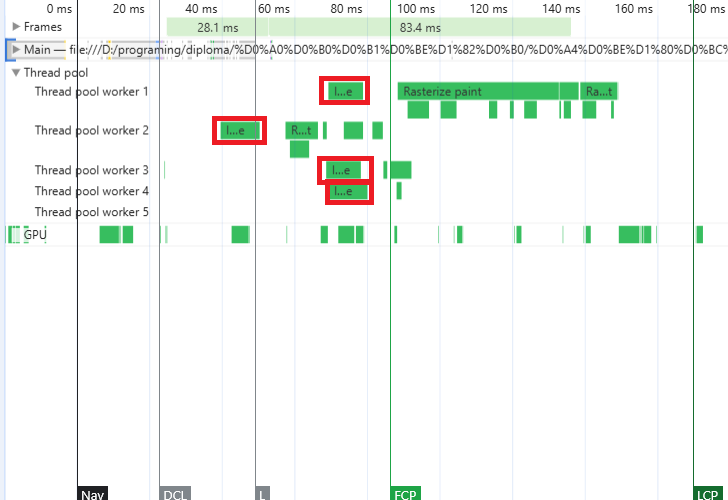
\includegraphics[width=1\textwidth]{../images/image_comp/devtools.png}
    \caption{Диаграмма загрузки потоков}
\end{figure}

Красными прямоугольниками выделено время декодирования изображений.

На данной диаграмме мы видим временные интервалы соответствующие декодированию и растеризации изображений.
По оси X отложено время в миллисекундах, по оси Y представлены задействованные потоки процессора

Как можно заметить, браузер умеет декодировать изображения параллельно.

В основном реализуется следующая схема:

\begin{enumerate}
    \item Браузер скачивает файл
    \item Декодирует
    \item Отрисовывает
\end{enumerate}

Но, т.к JPEG поддерживает последовательное декодирование,
может получится так, что браузер сначала декодирует часть изображения,
растеризует декодированную часть, декодирует ещё одну часть и так далее.
На практике я наблюдал разбиение изображения на три части

Для изображения весом 344kB я получил время декодирования
$T_{dec}=13,4 \pm 1 \text{ мс}$, время растеризации: $T_{ras}=8,9 \pm 0,9 \text{ мс}$

Дела обстоят хуже с другими форматами. Браузер не даёт информации о
времени декодирования.

\begin{figure}[H]
    \centering
    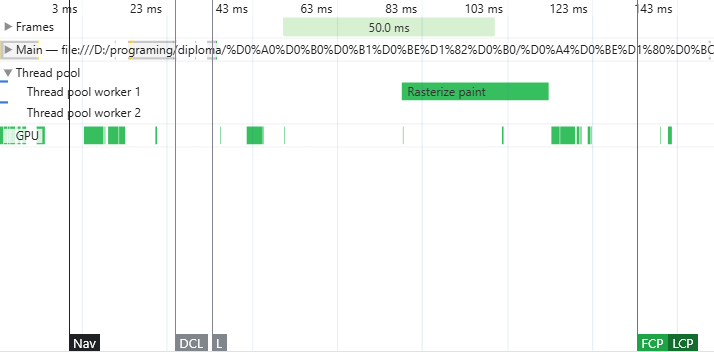
\includegraphics[width=1\textwidth]{../images/image_comp/avif_one_image.png}
    \caption{Диаграмма AVIF}
\end{figure}

Время растеризации для avif $T_{ras}=34,9 \pm 3,2\text{ мс}$, что заметно хуже чем у JPG

Мы можем измерить время, потраченное на декодирование + растеризацию косвенно.
Логично предположить, что $T_{LCP}$ измеряется по следующей формуле:

\[
    T_{LCP} = T_{\text{проч}} + T_{down} + T_{dec+ras}
\]

где:

\begin{itemize}
    \item $T_{\text{проч}}$ - время на рендеринг DOM, время на отправку
          запроса HTTP и прочие
          функции браузера, которые не зависят от формата
    \item $T_{dec+ras}$ - время на декодирование и растеризацию

    \item $T_{down}$ - время на загрузку файла, для JPEG $T_{down} = 1,3 \pm 0,2 \text{ мс}$,
          для PNG $T_{down} = 2,4 \pm 0,3 \text{ мс}$. Так как оно на порядок меньше $T_{dec+ras}$,
          им можно пренебречь
\end{itemize}

Тогда замерив $T_{LCP}$ для разных форматов, можно найти разность $T_{dec+ras}$.

\begin{table}[H]
    \centering
    \caption{Результаты измерений LCP}
    \begin{tabular}{l S[table-format=3.1] S[table-format=2.2]}
        \toprule
        Формат & {$\overline{T}_{\text{LCP}}$, \text{мс}} & {$\sigma$, \text{мс}} \\
        \midrule
        JPEG   & 73,5                                     & 8,05                  \\
        PNG    & 141,3                                    & 7,51                  \\
        AVIF   & 139,5                                    & 6,6                   \\
        WebP   & 125,3                                    & 6,51                  \\
        \bottomrule
    \end{tabular}
\end{table}

Считая, что для JPEG $T_{dec+ras} = 22,8 \pm 2 \text{ мс}$, получим:

\begin{table}[H]
    \centering
    \caption{Время декодирования и растеризации}
    \begin{tabular}{l S[table-format=2.1] S[table-format=1.2]}
        \toprule
        Формат & {$\overline{T}_{dec+ras}$, \text{мс}} & {$\sigma$, \text{мс}} \\
        \midrule
        JPEG   & 22,8                                  & 2,00                  \\
        PNG    & 90,6                                  & 9,51                  \\
        AVIF   & 88,8                                  & 8,6                   \\
        WebP   & 74,6                                  & 8,51                  \\
        \bottomrule
    \end{tabular}
\end{table}

Попробуем определить критерии оптимального формата с точки зрения LCP.
Предположим, у нас есть некоторое изображение.
Также у нас постоянные характеристики аппартой части клиента.
Тогда $T_{LCP}$ зависит только от двух параметров: $V_{down}$ и $i_{comp}$, где:

\begin{itemize}
    \item $V_{down}$ - скорость загрузки пользователя
    \item $i_{comp}$ - формат кодирования
\end{itemize}

Тогда:

\[
    T_{LCP} = T_{LCP}(V_{down}, i_{comp}) = T^{i}_{\text{проч}} + T^{i}_{down} + T^{i}_{dec+ras} = T_{\text{проч}} + \frac{M_{\text{исх}}}{k_{i}*V_{down}} + T^{i}_{dec+ras}
\]

$M_{\text{иск}}$ - исходный вес изображения в Мб\\
$k_i$ - степень сжатия\\

Используя эту формулу, найдём скорость загрузки пользователя, при которой $T^{JPEG}_{LCP} = T^{AVIF}_{LCP}$ для протестированного изображения:

\[
    T_{\text{проч}} + \frac{M_{\text{исх}}}{k_{JPEG}*V^{equal}_{down}} + T^{JPEG}_{dec+ras} = T_{\text{проч}} + \frac{M_{\text{исх}}}{k_{AVIF}*V^{equal}_{down}} + T^{AVIF}_{dec+ras}
\]

\begin{equation}
    V^{equal}_{down} = \frac{M_{\text{исх}}(k_{AVIF}-k_{JPEG})}{k_{JPEG}k_{AVIF}(T^{AVIF}_{dec+ras} - T^{JPEG}_{dec+ras})}
\end{equation}

$M_{\text{исх}} = 2,9\text{ Мб}$, $k_{JPEG} = 8,89$, $k_{AVIF} = 16,14$

\[
    V^{equal}_{down} = 17,76 \text{ мбит/c}
\]

Что вдвое быстрее скорости загрузки хорошего 4G.
Выше этой скорости будет эффективнее JPEG, ниже - AVIF.

Чтобы проверить теоретические расчёты, предлагаю сравнить $T_{LCP}$ у JPEG
и AVIF для разных скоростей:

\begin{itemize}
    \item Fast 4G 7,5 мбит/c
    \item «Double» 4G 18 мбит/c
    \item Без замедления
\end{itemize}

\begin{table}[H]
    \centering
    \caption{Сравнение LCP для разных скоростей}
    \begin{tabular}{l S[table-format=3.2] S[table-format=2.2]}
        \toprule
        Формат              & {$\overline{\text{LCP}}$, \si{\milli\second}} & {$\sigma$, \si{\milli\second}} \\
        \midrule
        Fast 4G, JPEG       & 799                                           & 20                             \\
        Fast 4G, AVIF       & 736                                           & 13                             \\
        «Doble» 4G JPEG     & 689                                           & 23                             \\
        «Doble» 4G AVIF     & 689                                           & 15                             \\
        Без замедления JPEG & 151                                           & 5                              \\
        Без замедления AVIF & 198                                           & 25                             \\
        \bottomrule
    \end{tabular}
\end{table}

Измерения подтверждают выведенную формулу. Может возникнуть вопрос: почему в этом измерении без замедления, $LCP$ оказался больше чем в предыдущем опыте? .
Дело в сервере раздачи статических файлов, который позволил конфигурировать параметры сети.

Также стоит подметить, что LCP увеличился в случаях 4G и Double 4G из-за искусственной задержки ответа сервера,
что эмулирует реальную 4G сеть.

\subsubsection{Практические рекомендации }

Учитывая, что полученная $V^{equal}_{down} = 17,76 \text{мбит/c}$
соответсвует пограничной скорости мобильного интернета,
следует использовать формат AVIF, если целевая аудитория сайта - пользователи
мобильных устройств, и JPEG, если используются десктопные устройства (100мбит/c).
Конечно, в случае, когда нам не требуется поддержка прозрачности.
В противном случае рекомендуется использовать WebP.

\subsubsection{Случай с множеством изображений }

Когда на сайте несколько изображений, следует учитывать возможность
параллельного декодирования и растеризации, в этом случае $V^{equal}_{down}$
будет другой. Формула расчёта зависит от числа потоков, задействованных браузером.
В целом для нескольких изображений и многопоточных устройств из-за возможности
параллельно декодировать и отрисовывать изображения $V^{down}_{equal}$ получается
в несколько раз выше.

\subsection{Сжатие статических файлов браузера с помощью Gzip, Brotli}

Приступим к измерению показателей методов сжатия без потерь. Но перед этим хочу
акцентировать внимание на формуле, для вычисления полного времени скачивания
сжатых данных

\begin{equation}
    T_{\text{полн}} = T_{\text{comp}} + T_{down} + T_{decomp}
\end{equation}

где:

\begin{itemize}
    \item $T_{\text{comp}}$ - время сжатия данных, для статических файлов $T_{\text{comp}}=0$
    \item $T_{down}$ - время скачивания сжатого тела запроса, зависит от степени сжатия
    \item $T_{decomp}$ - время декомпрессии
\end{itemize}

\subsubsection{Что измеряем}

Для алгоритмов gzip, brotli будут измерены:

\begin{itemize}[label=-]
    \item Степень сжатия
    \item Время сжатия
    \item Время декомпрессии
\end{itemize}

В качестве исходных данных будут использованы минифицированные версии трёх веб-приложений:

\begin{itemize}[label=-]
    \item Dating App (DA)
    \item Videohosting (VH)
    \item Angular conduit (AC)
\end{itemize}

\subsubsection{Технические характеристики устройства}

Процессор: Intel(R) Core(TM) i5-10210U CPU @ 1.60GHz 2.11 GHz\\
Оперативная память: 8,00 ГБ\\
Операционная система: Windowws 11, версия 24H2, WSL Linux Ubuntu 20.04

\subsubsection{Условия проведения эксперимента, обработка данных}

Для сжатия методами Gzip, Brotli использована утилита gzipper на node.js

Для декопрессии использованы утилиты gunzip, brotli на Linux

Для замеров времени декомпрессии использован hyperfine

Построены минимумы по времени

Для точности измерений были отключены фоновые процессы операционной системы

В веб-приложениях были удалены файлы с изображениями, т.к они уже сжаты с помощью специальных алгортмов для изображений (jpg, webp, avif)

Изначальный размер приложений:

\begin{itemize}
    \item Dating App (DA) 999КБ
    \item Videohosting (VH) 479КБ
    \item Angular conduit (AC) 456КБ
\end{itemize}

\subsubsection{Измерение степени сжатия}

\begin{figure}[H]
    \centering
    \begin{minipage}{0.48\textwidth}
        \centering
        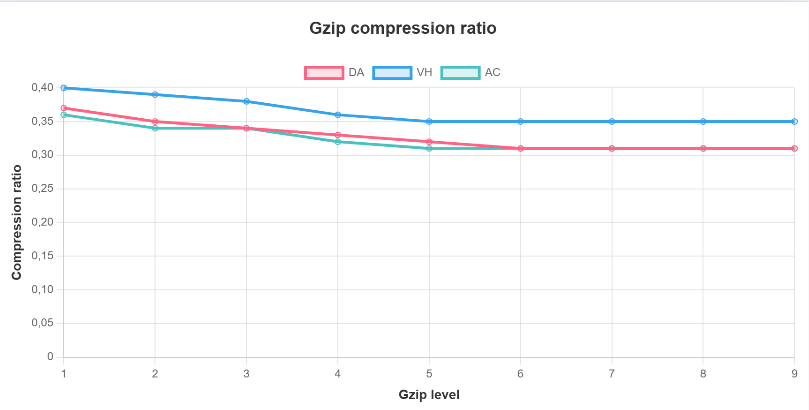
\includegraphics[width=\linewidth]{../images/gzip_compress_ratio.png}
        \caption{Степень сжатия Gzip}
        \label{fig:image1}
    \end{minipage}
    \hfill
    \begin{minipage}{0.48\textwidth}
        \centering
        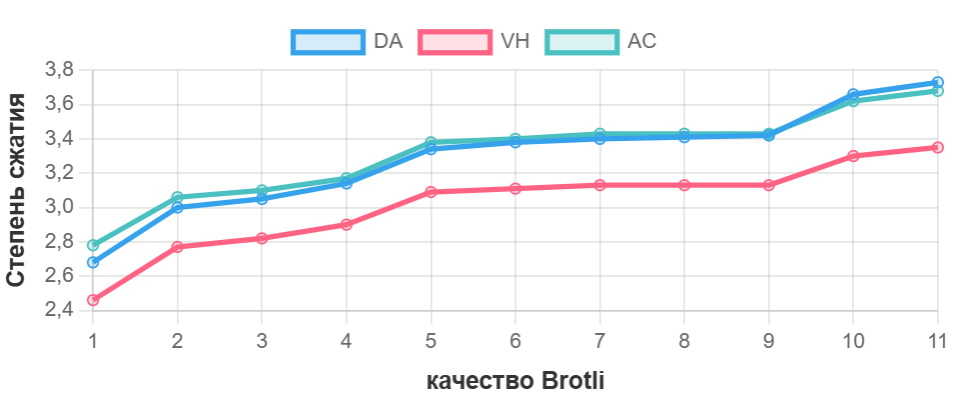
\includegraphics[width=\linewidth]{../images/brotli_compressed_ratio.png}
        \caption{Степень сжатия Brotli}
        \label{fig:image2}
    \end{minipage}
\end{figure}

\subsubsection{Измерение времени сжатия}

\begin{figure}[H]
    \centering
    \begin{minipage}{0.48\textwidth}
        \centering
        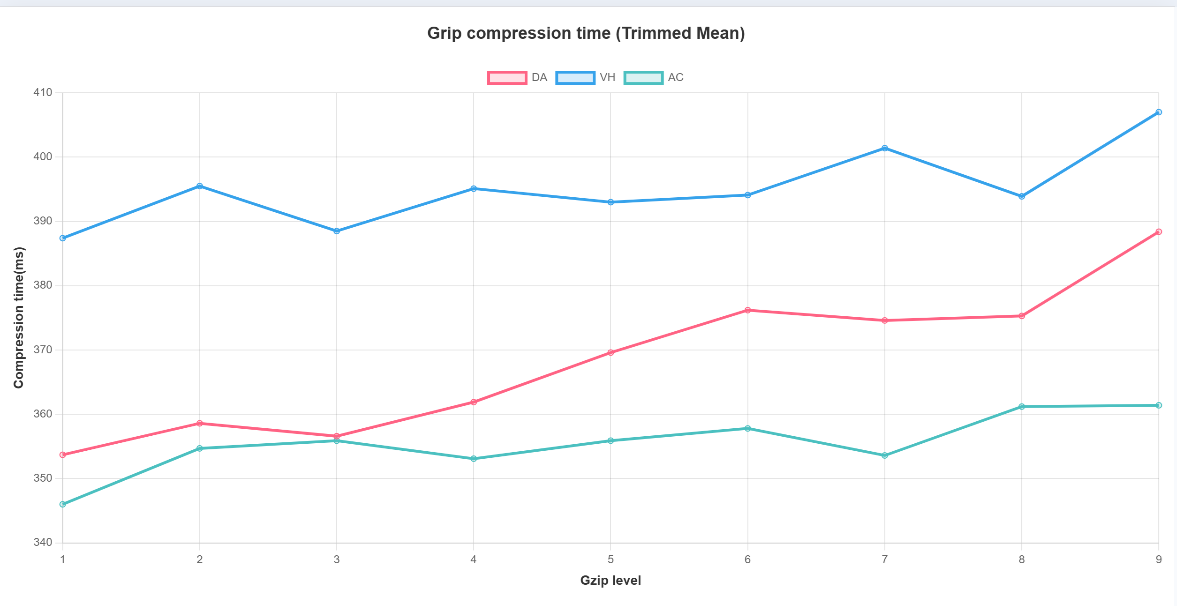
\includegraphics[width=\linewidth]{../images/Gzip compression time (Trimmed Mean).png}
        \caption{Время сжатия Gzip}
        \label{fig:image1}
    \end{minipage}
    \hfill
    \begin{minipage}{0.48\textwidth}
        \centering
        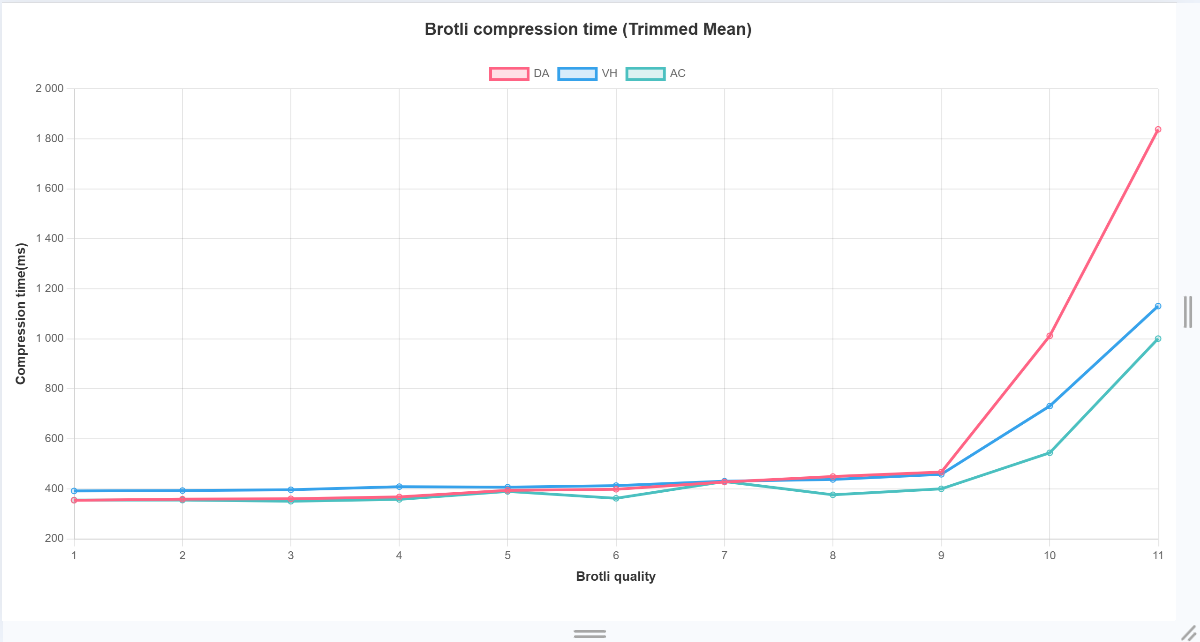
\includegraphics[width=\linewidth]{../images/Brotli compression time (Trimmed Mean).png}
        \caption{Время сжатия Brotli}
        \label{fig:image2}
    \end{minipage}
\end{figure}

Было замечено, что gzipper тратит 160ms на пустой файл, вероятно это время требуется, чтобы запустить процесс,
выделить память. Поэтому также построены графики за вычетом времени на накладные расходы

\begin{figure}[H]
    \centering
    \begin{minipage}{0.48\textwidth}
        \centering
        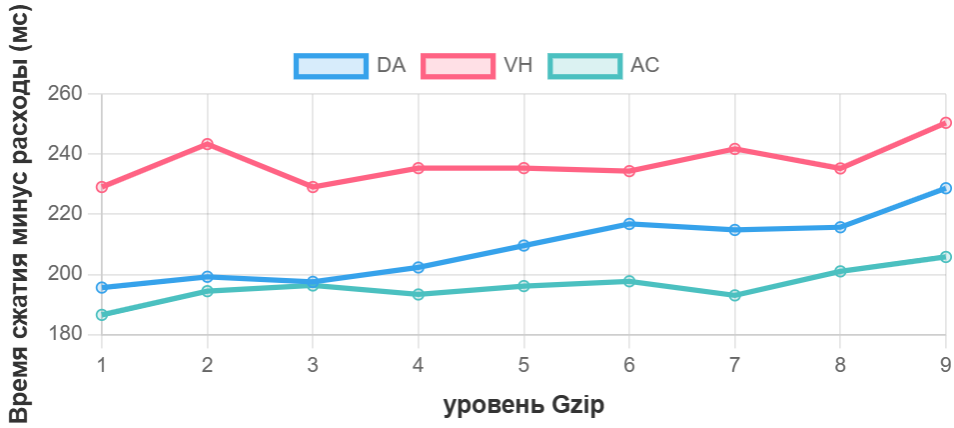
\includegraphics[width=\linewidth]{../images/Gzip compression time (min-overhead).png}
        \caption{Время сжатия Gzip за вычетом накладных расходов}
        \label{fig:image1}
    \end{minipage}
    \hfill
    \begin{minipage}{0.48\textwidth}
        \centering
        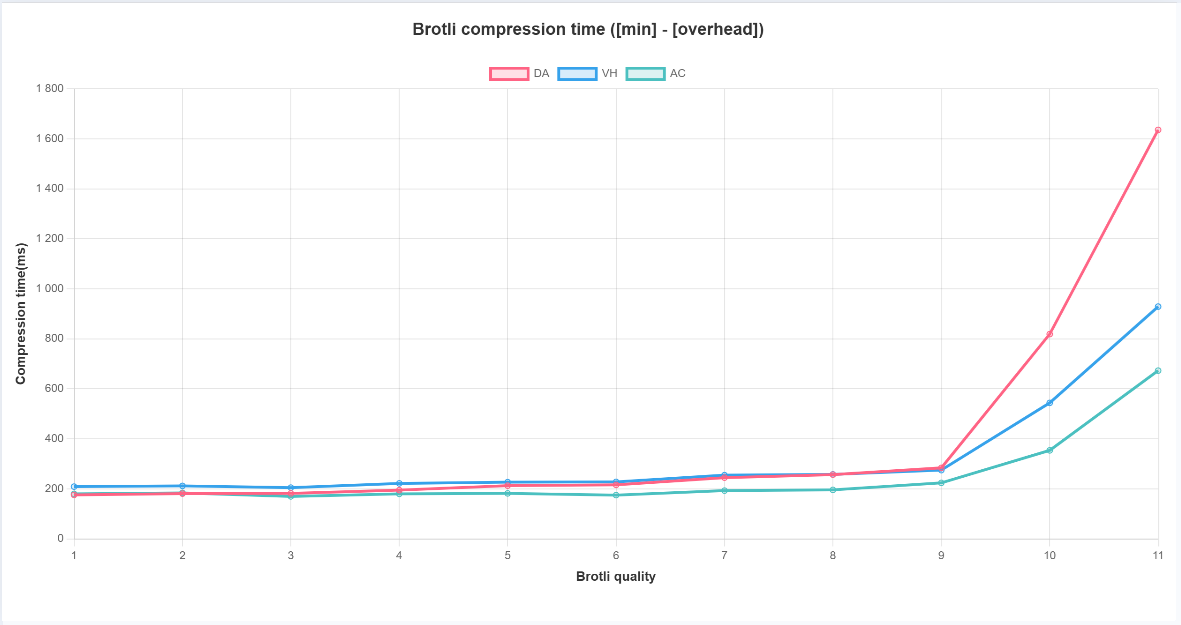
\includegraphics[width=\linewidth]{../images/Brotli compression time (min-overhead).png}
        \caption{Время сжатия Brotli за вычетом накладных расходов}
        \label{fig:image2}
    \end{minipage}
\end{figure}

Как можно заметить, время сжатия для Gzip почти не зависит от степени сжатия, как следствие, можно пробовать сжимать динамические данные, приминяя максимальный уровень.

У Brotli выделяются только два последних уровня, алгоритм тратит время кратно больше.
Для динамиских данных лучше использовать уровни с 5-го по 9-й.

\subsubsection{Измерение времени декомпрессии}

Измерения времени декомпрессии программой gunzip произведены на Ubuntu Linux 24.04. Для замеров использована утилита hyperfine.

\begin{figure}[H]
    \centering
    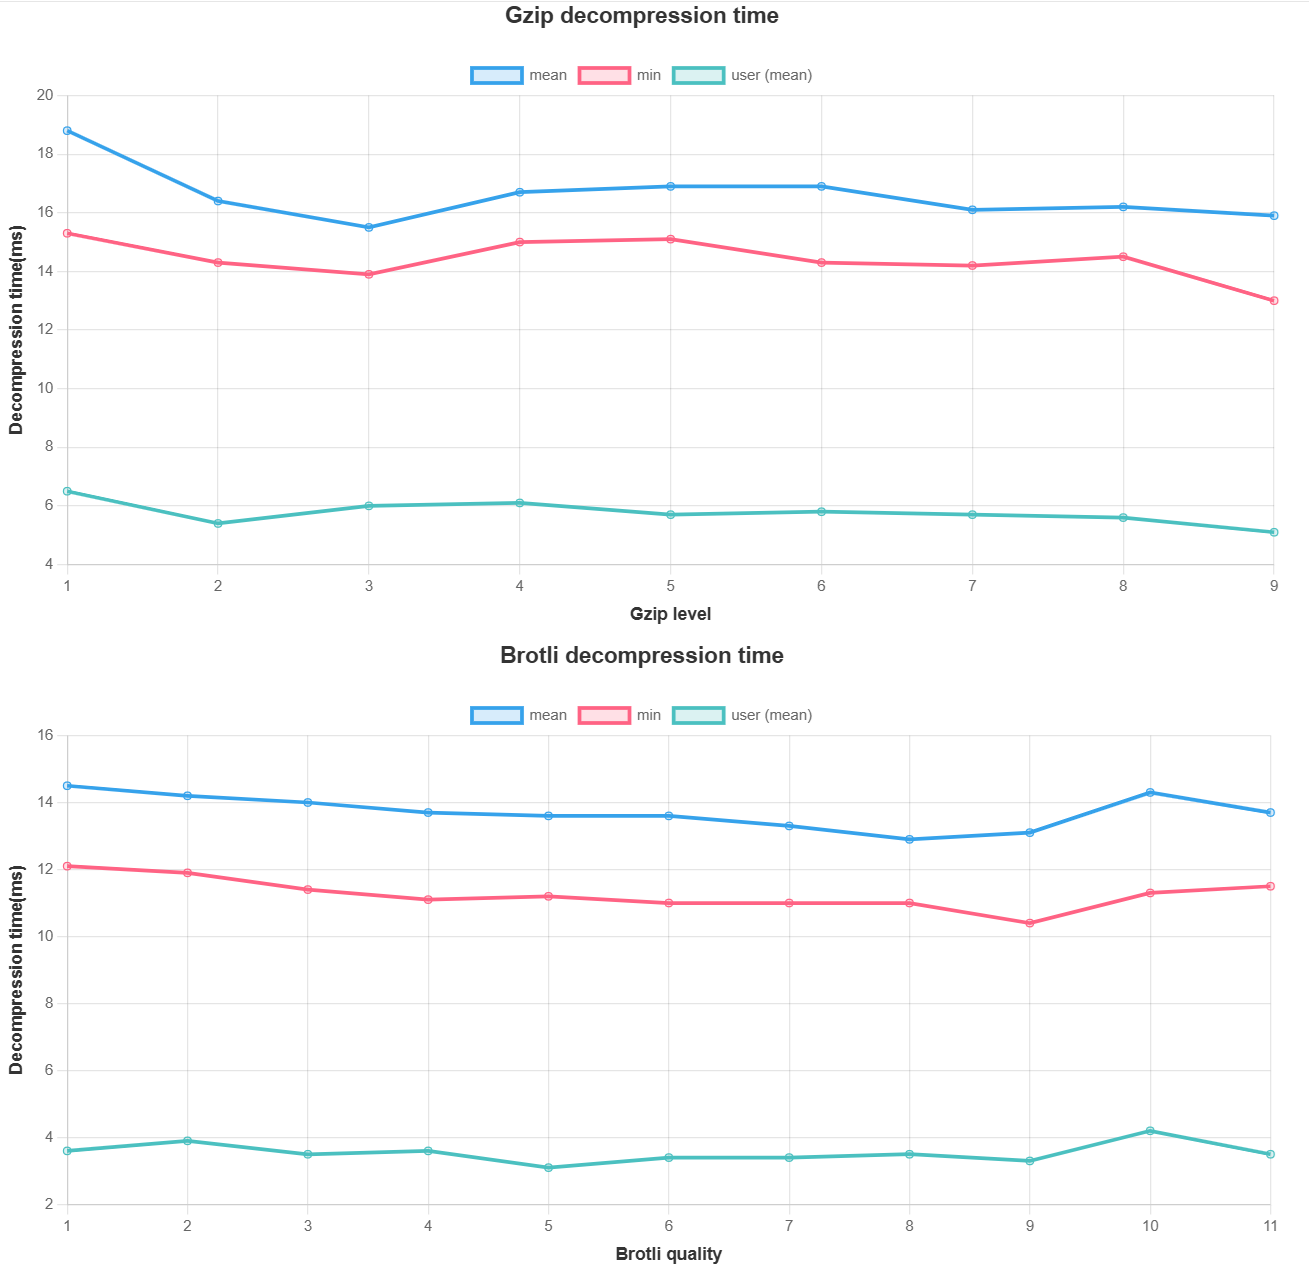
\includegraphics[width=1\textwidth]{../images/Decompression_time.png}
    \caption{Рисунок 22}
\end{figure}

Как видно из графика, скорость декомпрессии почти не зависит от степени сжатия. Это следует из ассиметричности алгоритмов семейства LZ77.
Напрашивается вывод, что статические данные стоит сжимать максимально, как только возможно.
Также стоит отметить, что brotli в среднем быстрее разжимает файлы чем gzip (имеются в виду конкретные программы).

Итак, проанализировав результаты измерений, мы сделали выводы по практическому применению, исходя из формулы (2).
Посмотрим к каким результам мы придём, произведя замеры в консоли браузера для классического сценария работы пользователя. 

\subsection{Реальные замеры сжатия статических файлов в браузере}

\subsubsection{Постановка эксперимента}

Смоделируем ситуацию, когда пользователь заходит на сайт и для продолжения работы ему нужно загрузить статические файлы (JS, CSS).

Для напишем следующий index.html:

\begin{lstlisting}[language=HTML]
  <body>
    <script src="http://localhost:88/main.js" />
    <script>
      fetch("http://localhost:88/test");
    </script>
  </body>
\end{lstlisting}

Как это работает:

\begin{enumerate}
    \item Загружаем html документ
    \item Парсим html документ
    \item Встречаем \verb|<script src="http://localhost:88/main.js" />|, что говорит нам: загрузи и исполни скрипт с адреса "http://localhost:88/main.js",
          дальше не пойдём, пока этот скрипт не загрузится. В это время как раз входит время, необходимое на скачивание и декодирование.
          Скрипт я закомментировал, чтобы не испортить измерения сторонними вычислениями.
    \item Дальше выполняем запрос на "http://localhost:88/test". Это служит в качестве маркера. Время отправки запроса мы и будем измерять.
\end{enumerate}

Найду время отправки запроса для сжатия brottli 11x и для файла без сжатия. Может получиться так, что без сжатия будет быстрее,
так как не потребуется тратить время на декодировние.

Но т.к есть подозрения, что CPU throttling не влияет на время декодирования, также проведу замеры на своём мобильном телефоне Xiaomi 9T PRO в локальной сети Wi-Fi (300 Mb/s).

Так же дополнительно отключил кеширование на стороне клиента с помощью заголовков "Cache-Control", "Pragma"

Как и в прошлый раз ограничиваю фоновые процессы. 20 замеров на каждую характеристику

Время test запроса в случае с телефоном измерялось на стороне сервера.

\begin{itemize}
    \item $T_{gzip9}=65,35$мс, $\sigma = 9,21$мс
    \item $T_{no comress}=145,10$мс, $\sigma = 34,34$мс
\end{itemize}

\subsubsection{Вывод по статическим файлам JS, CSS, HTML}

Результаты измерений показали, что для статических файлов во всех случаях сжатия файлов либо существенно уменьшает время отклика, либо не увеличивает его.

То есть для любых устройств и любых параметров сети сжатие статических файлов будет предпочтительно, причём следует выбирать максимальную степень сжатия будь то gzip 9 или brotli 11

На данном этапе мы разобрались со статическими файлами. Теперь перейдём к динамическим данным, меняющимся с течением времени. Основное отличие состоит в том, что мы не можем сжать данные заранее, приходится применять сжатие "на лету". Наша задача  выяснить, как сжатие влияет на такие показатели, как:

\begin{itemize}
    \item Количество запросов в секунду (RPS)
    \item Нагрузка на сеть
    \item Время ожидание ответа от сервера
    \item Время загрузки содержимого запроса
    \item Общее время запроса
\end{itemize}

\subsection{Нагрузочное тестирование REST запросов (динамические данные)}

\subsubsection{Описание аппаратной части сервера}

Технические характеристики сервера:

\begin{itemize}
    \item CPU 1 vCPU
    \item RAM 2 Гб
    \item Storage 20 Гб
    \item Скорости загрузки, раздачи 1200 мб/c
\end{itemize}

Технические характеристика моего ноутбука:

\begin{itemize}
    \item CPU 4 ядра
    \item RAM 8 GB
    \item Скорости загрузки, раздачи 50 мб/c
\end{itemize}

В качестве REST сервера используется Node.js express.js, обратный прокси сервер (сжатие http) Nginx

Логика следующая:

\begin{enumerate}
    \item клиент заходит на сайт
    \item скачивает статические файлы
    \item когда выполнится js код, выполнится get запрос на получение всех видео /videos/getAll
    \item сервер сделает запрос в базу данных
    \item возвращает ответ
\end{enumerate}

Тестрирование проводится с помощью k6. Замеряются такие параметры, как:

\begin{itemize}
    \item Загрузка ЦП сервера
    \item Использование оперативной памяти сервера
    \item Время ожидание ответа от сервера
    \item Время загрузки содержимого запроса
    \item Процент успешно выполненных HTTP запросов
\end{itemize}

В зависимости от количества запросов в секунду (RPS)

Ответ от сервера представляет собой массив JSON:

\begin{lstlisting}[language=JavaScript]
[
  {
    title: "Steel Horizon",
    description:
      '"Steel Horizon" is a captivating cinematic journey that explores the boundaries of imagination and reality.
        With stunning visuals and a compelling narrative, it draws viewers into a richly woven tale full of emotion, suspense,
        and intrigue. As the characters navigate through complex challenges, deep personal struggles,
        and unexpected twists, the story unfolds with intensity and grace. Crafted by visionary creators,
        the film blends elements of classic storytelling with modern cinematic techniques to create an unforgettable experience.
        Whether you\'re drawn to heartfelt drama, thrilling action, or thought-provoking ideas,
        this film offers a powerful reflection on humanity, resilience, and discovery.',
    number: 19,
    src_url: "https://cdn.example.com/videos/video_19.mp4",
    preview_url: "/previews/bearwolf.mp4",
    image_url: "/images/bearwolf2.jpg",
    studios: ["MegaPix"],
    tags: ["documentary", "action", "comedy"],
  }
]
\end{lstlisting}

\subsubsection{ Физический смысл выбранной нагрузки }

\begin{figure}[H]
    \centering
    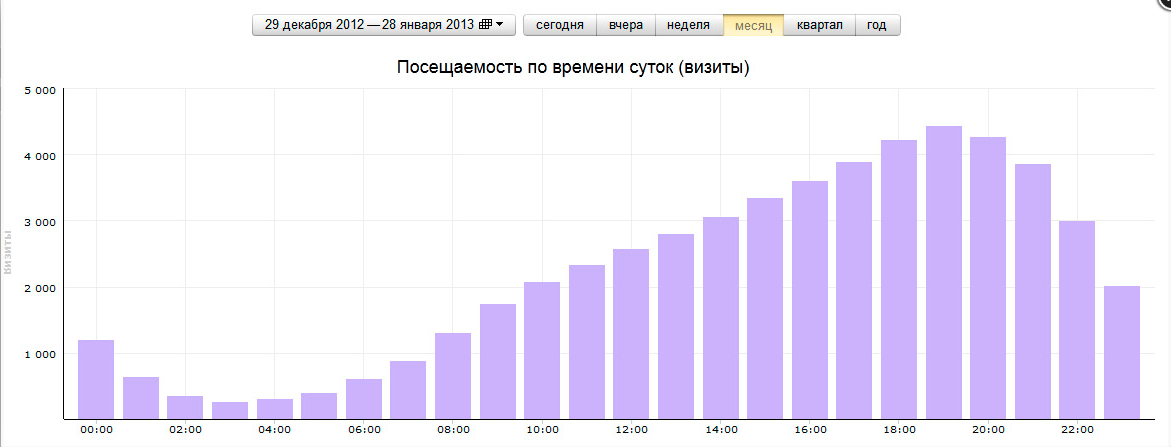
\includegraphics[width=1\textwidth]{../images/pedsovet.png}
    \caption{Количество посещений в час}
\end{figure}

Перед вами статистика посещаемости некоторого сайта за день. Собрано количество посещений за каждый час и построена гистограмма.
Можно заметить неравномерность визитов в течение дня. Так в период с 18:00 до 19:00 количество посещений составило в районе 4000,
а с 2:00 до 3:00 менее 500. Это связано с территориальной распределённостью пользователей.
Если сайт русскоязычный, то логично предположить, что пик будет приходится на вечернее время по Москве,
так как население России преимущественно находится в её европейской части.
Поэтому важно узнать, как ведёт себя сервер при разной нагрузке.

Было проведено два эксперимента соответствующие пиковой и умеренной нагрузке.
Предполагается, что в условиях средне-низкой нагрузки, когда у ЦП есть достаточно ресурсов,
сжатие проявит себя лучше, чем в условиях нехватки мощностей.

\subsubsection{Эксперимент первый}

Нагрузка:

\begin{lstlisting}[language=JavaScript]
  stages: [
    { duration: "5s", target: 10 },
    { duration: "10s", target: 20 },
    { duration: "10s", target: 30 },
    { duration: "10s", target: 40 },
    { duration: "10s", target: 50 },
    { duration: "10s", target: 60 },
    { duration: "10s", target: 70 },
    { duration: "10s", target: 80 },
    { duration: "10s", target: 90 },
    { duration: "10s", target: 100 },
    { duration: "10s", target: 110 },
    { duration: "10s", target: 120 },
    { duration: "10s", target: 130 },
    { duration: "10s", target: 140 },
    { duration: "10s", target: 150 },
    { duration: "10s", target: 170 },
    { duration: "10s", target: 190 },
    { duration: "10s", target: 210 },
    { duration: "5s", target: 5 },
  ]
\end{lstlisting}

duration - время каждой стадии, target - кол-во одновременно активных пользователей
Каждый пользователь отправляет запрос на сервер, ждёт ответа, далее ждёт 1 секунду и отправляет запрос снова.

\begin{table}[h]
    \centering
    \caption{Результаты без сжатия}
    \begin{tabular}{lr}
        \toprule
        \textbf{Метрика}                          & \textbf{Значение}               \\
        \midrule
        Всего проверок (checks\_total)            & 4662                            \\
        \hline
        Среднее время получения (receiving\_time) & \SI{2660}{\milli\second}        \\
        Минимальное время получения               & \SI{187}{\milli\second}         \\
        Медианное время получения                 & \SI{2388}{\milli\second}        \\
        Максимальное время получения              & \SI{45987}{\milli\second}       \\
        \hline
        Среднее общее время (total\_duration)     & \SI{2770}{\milli\second}        \\
        Медианное общее время                     & \SI{2492}{\milli\second}        \\
        90-й персентиль общего времени            & \SI{5476}{\milli\second}        \\
        \hline
        Среднее время ожидания (waiting\_time)    & \SI{106}{\milli\second}         \\
        \hline
        Средняя продолжительность HTTP-запроса    & \SI{2.7}{\second}               \\
        90-й персентиль HTTP-запросов             & \SI{5.47}{\second}              \\
        \hline
        Получено данных (Network data received)   & \SI{4.9}{\mega\byte\per\second} \\
        \bottomrule
    \end{tabular}
\end{table}

\begin{table}[h]
    \centering
    \caption{Результаты без сжатия}
    \begin{tabular}{lS[table-format=5.5]}
        \toprule
        \textbf{Метрика} & \textbf{Время (\si{\milli\second})} \\
        \midrule
        P50 (медиана)    & 2388                                \\
        P90              & 5320                                \\
        P95              & 6528                                \\
        Максимум         & 46186                               \\
        \bottomrule
    \end{tabular}
\end{table}

\begin{table}[h]
    \centering
    \caption{Результаты с сжатием (gzip 9)}
    \begin{tabular}{lr}
        \toprule
        \textbf{Метрика}                          & \textbf{Значение}               \\
        \midrule
        Всего проверок (checks\_total)            & 10324                           \\
        Частота проверок                          & \SI{57.0}{\per\second}          \\
        \hline
        Среднее время получения (receiving\_time) & \SI{1.45}{\milli\second}        \\
        Минимальное время получения               & \SI{6}{\milli\second}           \\
        Медианное время получения                 & \SI{1.00}{\milli\second}        \\
        Максимальное время получения              & \SI{592}{\milli\second}         \\
        \hline
        Среднее общее время (total\_duration)     & \SI{671}{\milli\second}         \\
        Медианное общее время                     & \SI{609}{\milli\second}         \\
        90-й персентиль общего времени            & \SI{1511}{\milli\second}        \\
        \hline
        Среднее время ожидания (waiting\_time)    & \SI{670}{\milli\second}         \\
        \hline
        Средняя продолжительность HTTP-запроса    & \SI{671}{\milli\second}         \\
        90-й персентиль HTTP-запросов             & \SI{1515}{\milli\second}        \\
        \hline
        Получено данных (Network data received)   & \SI{339}{\kilo\byte\per\second} \\
        \bottomrule
    \end{tabular}
\end{table}

\begin{table}[H]
    \centering
    \caption{Результаты с сжатием (gzip 9)}
    \begin{tabular}{lS[table-format=4.5]}
        \toprule
        \textbf{Метрика} & \textbf{Время (\si{\milli\second})} \\
        \midrule
        P50 (медиана)    & 609                                 \\
        P90              & 1511                                \\
        P95              & 1721                                \\
        Максимум         & 1958                                \\
        \bottomrule
    \end{tabular}
\end{table}

\subsubsection{Эксперимент второй}

Нагрузка:

\begin{lstlisting}[language=JavaScript]
   stages: [
    { duration: "10s", target: 10 },
    { duration: "20s", target: 10 },
    { duration: "20s", target: 15 },
    { duration: "20s", target: 20 },
    { duration: "20s", target: 25 },
    { duration: "20s", target: 30 },
    { duration: "10s", target: 5 },
  ]
\end{lstlisting}

\begin{table}[h]
    \centering
    \caption{Метрики производительности (без сжатия, эксперимент 2)}
    \label{tab:metrics}
    \begin{tabular}{lS[table-format=4.3]}
        \toprule
        \textbf{Метрика}                          & \textbf{Значение}               \\
        \midrule
        \multicolumn{2}{l}{\textbf{Основные показатели}}                            \\
        Всего проверок (checks\_total)            & 1454                            \\
        Частота проверок                          & \SI{12.0}{\per\second}          \\
        Скорость получения данных                 & \SI{2.5}{\mega\byte\per\second} \\
        \hline
        \multicolumn{2}{l}{\textbf{Временные характеристики}}                       \\
        Среднее время получения (receiving\_time) & 309.4\ мс                       \\
        Медианное время получения                 & 266.4\ мс                       \\
        Максимальное время получения              & 1099.2\ мс                      \\
        \hline
        Среднее общее время (total\_duration)     & 380.0\ мс                       \\
        Медианное общее время                     & 338.6\ мс                       \\
        90-й персентиль общего времени            & 518.7\ мс                       \\
        \hline
        Среднее время ожидания (waiting\_time)    & 70.5\ мс                        \\
        Медианное время ожидания                  & 69.4\ мс                        \\
        \hline
        Среднее время HTTP-запроса                & 380.0\ мс                       \\
        90-й персентиль HTTP-запросов             & 518.7\ мс                       \\
        \bottomrule
    \end{tabular}
\end{table}

\begin{table}[h]
    \centering
    \caption{Метрики производительности (gzip-9, эксперимент 2)}
    \begin{tabular}{lS[table-format=3.3]}
        \toprule
        \textbf{Метрика}                          & \textbf{Значение}              \\
        \midrule
        \multicolumn{2}{l}{\textbf{Основные показатели}}                           \\
        Всего проверок (checks\_total)            & 1861                           \\
        Частота проверок                          & \SI{15.4}{\per\second}         \\
        Скорость получения данных                 & \SI{92}{\kilo\byte\per\second} \\
        \hline
        \multicolumn{2}{l}{\textbf{Временные характеристики (мс)}}                 \\
        Среднее время получения (receiving\_time) & 1.77                           \\
        Медианное время получения                 & 1.72                           \\
        Максимальное время получения              & 65.9                           \\
        \hline
        Среднее общее время (total\_duration)     & 75.3                           \\
        Медианное общее время                     & 74.4                           \\
        90-й персентиль общего времени            & 81.0                           \\
        \hline
        Среднее время ожидания (waiting\_time)    & 73.4                           \\
        Медианное время ожидания                  & 72.6                           \\
        \hline
        Среднее время HTTP-запроса                & 75.3                           \\
        90-й персентиль HTTP-запросов             & 81.0                           \\
        \bottomrule
    \end{tabular}
\end{table}

\subsubsection{Анализ полученных результатов }

В первом эксперименте с пиковой нагрузкой прирост в количестве обработанных запросов составил 121\%, во втором - 28\%.
Заметим, что с ростом числа пользователей, несмотря на чудовищные по меркам сайтов $T_{req}=2,6$c,
сервер не отклоняет запросы, а ставит их в очередь. Максимальная длина очереди - число пользователей.
Пусть $V_{max}$ - максимальное число запросов, которое сервер может обработать в секунду.
Найдём $T_{req}$ в \textbf{установившемся пиковом} режиме.
Условие установившегося режима - количество поступающих запросов совпадает с количеством обработанных:

\[
    \frac{N_{users}}{T_{req} + T_{wait}}=V_{\text{max}}
\]

\[
    T_{req} = \frac{N_{users}}{V_{\text{max}}} - T_{wait}
\]

Из этой формулы можно найти максимальное число пользователей, при котором начнут отклоняться http запросы:

\begin{equation}
    N^{\text{крит}}_{users} = (T^{\text{крит}}_{req} + T_{wait}){V_{\text{max}}}
\end{equation}

Так, для $T^{\text{крит}}_{req} = 10$с, $T_{wait}=1$c, $V_{max}=80$RPS, $N^{\text{крит}}_{users}=880$

В первом эксперименте обе конфигурации вышли на пиковый режим. В случае без сжатия узким горлышком оказалась сеть, во втором - мощность процессора.

\subsubsection{Зависимость CPU load, Network load от уровня сжатия}

Ограничение на скорость создано искусственно с помощью настройки роутера QoS, максимальная скорость около 200 Mb/s\\
Ограничие скорости гарантирует постоянную полосу пропускания\\
На сервере отключены все построронние процессы. CPU используется только для:

\begin{itemize}
    \item MySQL Database
    \item Backend server (Express.js)
    \item Обратный прокси сервер (Nginx)
\end{itemize}

Нагрузка:

\begin{lstlisting}[language=JavaScript]
  stages: [
    { duration: "5s", target: 10 },
    { duration: "10s", target: 20 },
    { duration: "10s", target: 30 },
    { duration: "10s", target: 40 },
    { duration: "10s", target: 50 },
    { duration: "10s", target: 60 },
    { duration: "10s", target: 70 },
    { duration: "10s", target: 80 },
    { duration: "10s", target: 90 },
    { duration: "10s", target: 100 },
    { duration: "10s", target: 110 },
    { duration: "10s", target: 120 },
    { duration: "10s", target: 130 },
    { duration: "10s", target: 140 },
    { duration: "10s", target: 150 },
    { duration: "10s", target: 170 },
    { duration: "10s", target: 190 },
    { duration: "10s", target: 210 },
    { duration: "5s", target: 5 },
  ]
\end{lstlisting}

В базе данных находится 400 видео, для тестирования используется Get запрос:
\verb|/video/getRecomendations/1|, который возвращает 100 случайных видео из базы данных. Около 100 видео, нужно для реализации корректного
скроллинга. (В одной строке можно разместить 5 видео, На экране помещается 5 строк, хотим закрыть
потребность в 3 скролах без подзагрузки, получаем 100 видео).

Будет варироваться степень сжатия:
\begin{itemize}
    \item no compress
    \item gzip 1
    \item gzip 5
    \item gzip 9
\end{itemize}

При построении графиков использовалось сглаживание по трём точкам

\[
    x^{smooth}_{i} = \frac{x_{i-1} + x_{i} + x_{i+1}}{3}
\]

Построены графики от времени

Результаты измерений:

\begin{table}[h]
    \centering
    \caption{Метрики производительности (без сжатия)}
    \begin{tabular}{lr}
        \toprule
        \textbf{Метрика}                       & \textbf{Значение}               \\
        \midrule
        Общее время теста                      & 3 минуты 01 секунда             \\
        \hline
        Всего проверок (checks\_total)         & 11827                           \\
        Частота проверок                       & \SI{65.3}{\per\second}          \\
        \hline
        Средняя продолжительность HTTP-запроса & \SI{456.3}{\milli\second}       \\
        Минимальное время ответа               & \SI{134.3}{\milli\second}       \\
        Медианное время ответа                 & \SI{232.7}{\milli\second}       \\
        Максимальное время ответа              & \SI{1.67}{\second}              \\
        90-й персентиль                        & \SI{1.13}{\second}              \\
        95-й персентиль                        & \SI{1.28}{\second}              \\
        \hline
        Объём полученных данных                & \SI{1.2}{\giga\byte}            \\
        Скорость получения данных              & \SI{6.9}{\mega\byte\per\second} \\
        \bottomrule
    \end{tabular}
\end{table}

\begin{table}[h]
    \centering
    \caption{Метрики производительности (gzip сжатие уровень 1)}
    \begin{tabular}{lr}
        \toprule
        \textbf{Метрика}                       & \textbf{Значение}               \\
        \midrule
        Общее время теста                      & 3 минуты                        \\
        \hline
        Всего проверок (checks\_total)         & 12745                           \\
        Частота проверок                       & \SI{70.3}{\per\second}          \\
        \hline
        Средняя продолжительность HTTP-запроса & \SI{350}{\milli\second}         \\
        Минимальное время ответа               & \SI{47.5}{\milli\second}        \\
        Медианное время ответа                 & \SI{146.1}{\milli\second}       \\
        Максимальное время ответа              & \SI{1.27}{\second}              \\
        90-й персентиль                        & \SI{994.4}{\milli\second}       \\
        95-й персентиль                        & \SI{1.07}{\second}              \\
        \hline
        Объём полученных данных                & \SI{57}{\mega\byte}             \\
        Скорость получения данных              & \SI{316}{\kilo\byte\per\second} \\
        \bottomrule
    \end{tabular}
\end{table}

\begin{table}[h]
    \centering
    \caption{Метрики производительности (gzip сжатие уровень 5)}
    \begin{tabular}{lr}
        \toprule
        \textbf{Метрика}                       & \textbf{Значение}               \\
        \midrule
        Общее время теста                      & 3 минуты                        \\
        \hline
        Всего проверок (checks\_total)         & 12338                           \\
        Частота проверок                       & \SI{68.1}{\per\second}          \\
        \hline
        Средняя продолжительность HTTP-запроса & \SI{396}{\milli\second}         \\
        Минимальное время ответа               & \SI{47.7}{\milli\second}        \\
        Медианное время ответа                 & \SI{157}{\milli\second}         \\
        Максимальное время ответа              & \SI{1.57}{\second}              \\
        99-й персентиль                        & \SI{1.05}{\second}              \\
        95-й персентиль                        & \SI{1.21}{\second}              \\
        \hline
        Объём полученных данных                & \SI{48}{\mega\byte}             \\
        Скорость получения данных              & \SI{266}{\kilo\byte\per\second} \\
        \bottomrule
    \end{tabular}
\end{table}

\begin{table}[h]
    \centering
    \caption{Метрики производительности (gzip сжатие уровень 9)}
    \begin{tabular}{lr}
        \toprule
        \textbf{Метрика}               & \textbf{Значение}               \\
        \midrule
        Общее время теста              & 3 минуты 01 секунда             \\
        \hline
        Всего проверок (checks\_total) & 12214                           \\
        Частота запросов               & \SI{67.4}{\per\second}          \\
        \hline
        Среднее время HTTP-запроса     & \SI{411.3}{\milli\second}       \\
        Минимальное время ответа       & \SI{44.3}{\milli\second}        \\
        Медианное время ответа         & \SI{338}{\milli\second}         \\
        Максимальное время ответа      & \SI{1.52}{\second}              \\
        90-й персентиль                & \SI{1.12}{\second}              \\
        95-й персентиль                & \SI{1.23}{\second}              \\
        \hline
        Объём полученных данных        & \SI{45}{\mega\byte}             \\
        Скорость передачи данных       & \SI{248}{\kilo\byte\per\second} \\
        \bottomrule
    \end{tabular}
\end{table}

\begin{figure}[H]
    \centering
    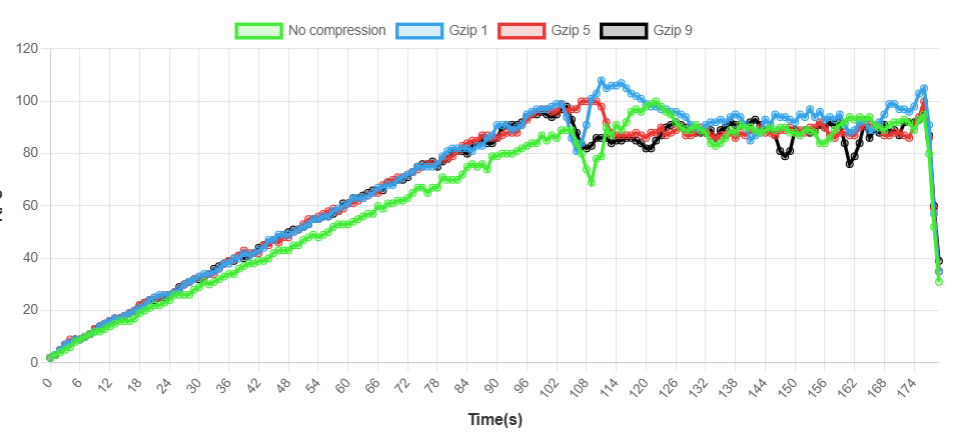
\includegraphics[width=1\textwidth]{../images/second_part/RPS.png}
    \caption{Количество запросов в секунду}
\end{figure}

\begin{figure}[H]
    \centering
    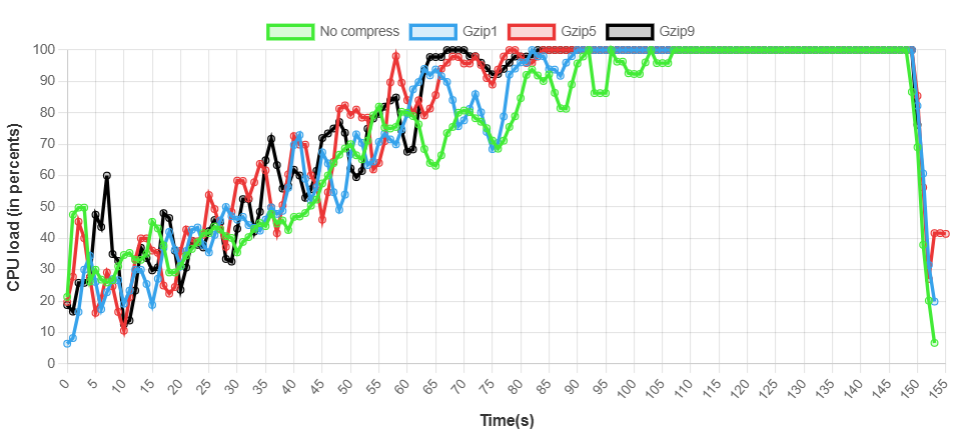
\includegraphics[width=1\textwidth]{../images/second_part/CPU_load.png}
    \caption{Загрузка CPU}
\end{figure}

\begin{figure}[H]
    \centering
    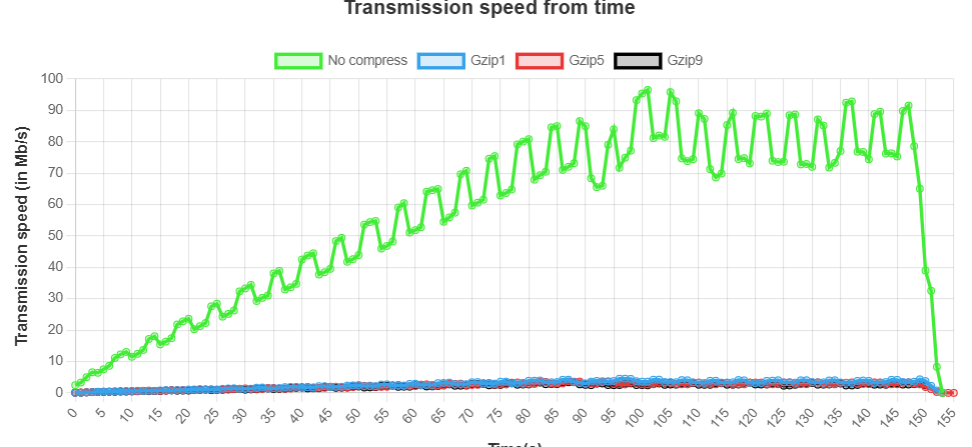
\includegraphics[width=1\textwidth]{../images/second_part/Transmission_speed.png}
    \caption{Загрузка сети}
\end{figure}

\begin{figure}[H]
    \centering
    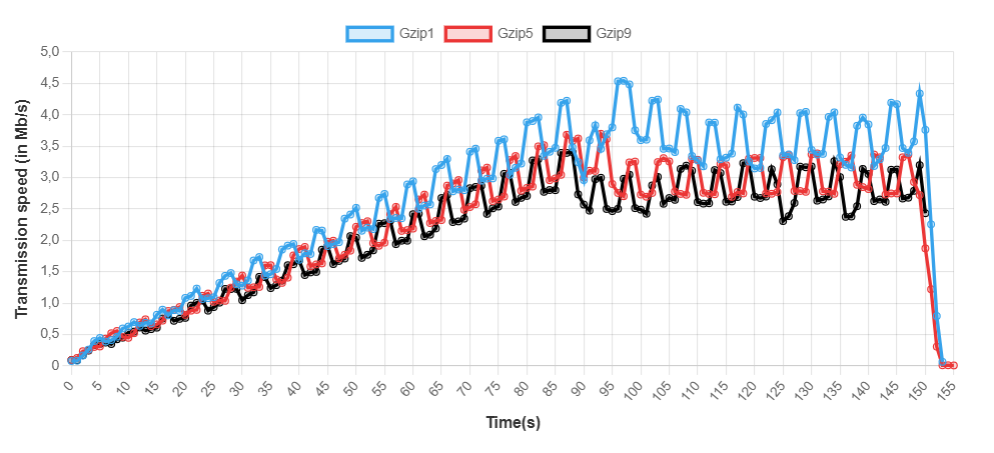
\includegraphics[width=1\textwidth]{../images/second_part/Transmission_speed_withot_nocompress.png}
    \caption{Загрузка сети только для сжатых запросов}
\end{figure}

\subsubsection{Анализ полученных результатов}

Нетрудно заметить, что использовние gzip заментно снизило нагрузку на сеть примерно в 20-30 раз,
при этом даже при 80 МБ/c несжатого трафика, нагрузка на CPU из-за сжатия оказалась крайне малой, что при загрузке CPU на 100\%,
показатель RPS остался на том же уровне.

Теперь выведем математические соотношения для нашей схемы эксперимента, из которых найдём оптимальные параметры сжатия.
Оптимальными будем считать такие параметры, при которых достигается максимум RPS.

\[
    V_{RPS} = V_{RPS}(N_{users}, i_{comp})
\]

где $N_{users}$ - количество активных пользователей, выполняющих запросы. $i_{comp}$ - уровень (качество, в случае Brotli) сжатия.

Рассмотрим сначала случай, когда у сервера всего один поток. Пусть на сервер пришёл один HTTP запрос, очередь пуста. Сервер последовательно выполнит следующие шаги:

\begin{enumerate}
    \item Принять HTTP запрос, аутентифицировать пользователя
    \item Сделать запрос в базу данных и подобрать персональные рекомендации,
    \item Применить сжатие к телу HTTP ответа
    \item Отправитть ответ пользователю
\end{enumerate}

В случае, если пользователей много, могут образовываться очереди. Одна очередь связана с обработкой ответа, вторая с загрузкой тела запроса.

\begin{figure}[H]
    \centering
    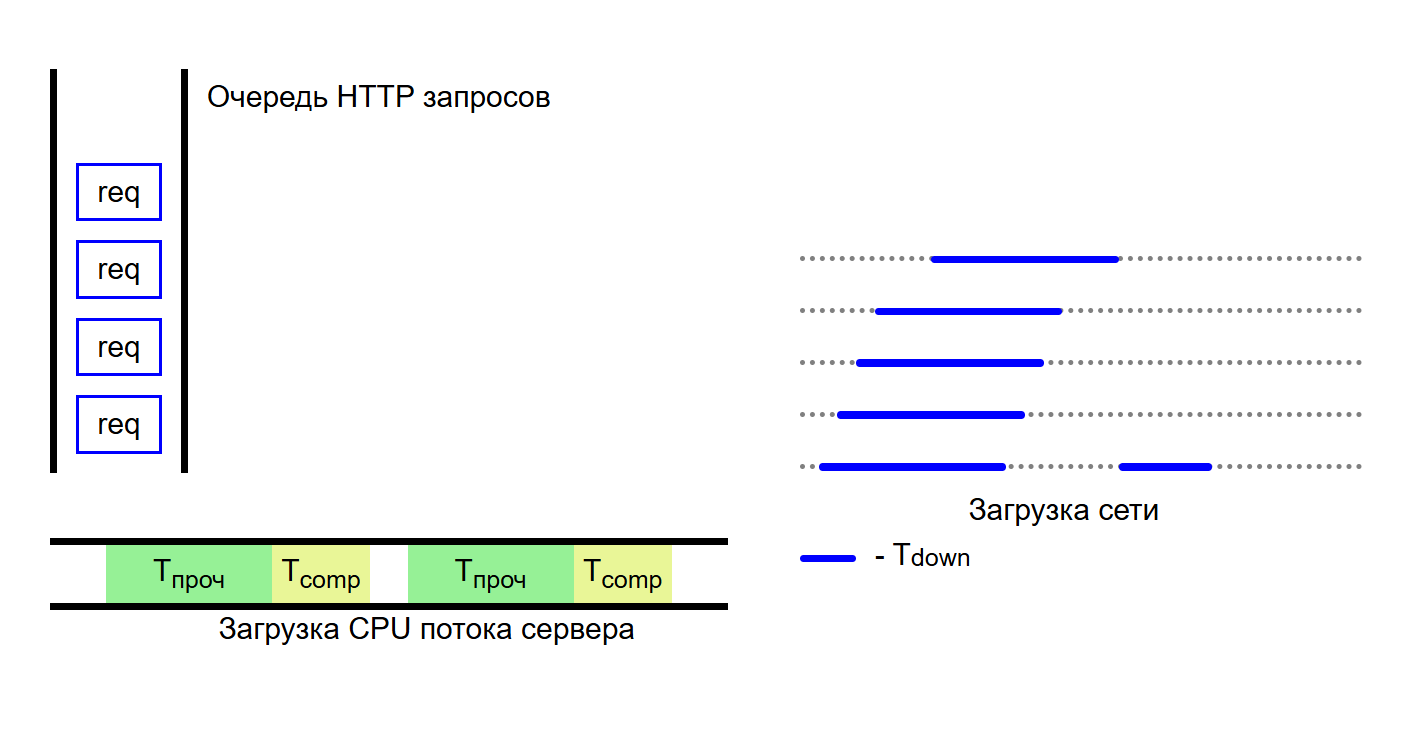
\includegraphics[width=1\textwidth]{../images/timing-model.png}
    \caption{Временная модель сервера}
\end{figure}

Если в данный момент в установившемся режиме $N \gg 1$ активных пользователей, можно ввести следующие характеристики:

\begin{itemize}
    \item $\overline{Q}_{HTTP}$ - среднее по времени число пользователей в очереди HTTP запросов,
    \item $\overline{Q}_{down}$ - среднее по времени число пользователей в очереди на скачивание,
\end{itemize}

RPS вычисляется по формуле:

\[
    RPS = \frac{N}{\overline{T}_{\text{полн}}}
\]

где $\overline{T}_{\text{полн}}$ - среднее полное время одного запроса:

Для конкретного запроса $T_{\text{полн}}$ рассчитывается по формуле:

\begin{equation}
    T_{\text{полн}} = T_{ping} + T_{\text{handle}}*(1 + Q_{HTTP}) + T_{down} + T_{decomp} + T_{wait}
\end{equation}

где:

\begin{itemize}
    \item $T_{ping}$ - время на сетевые задержки, связанные с удалённостью сервера и сетевым оборудования,
    \item $T_{\text{handle}} = T_{\text{проч} + T_{\text{сomp}}}$ - время на обработку одного запроса. В него входит время на аутентификацию, запрос к базе данных, сжатия тела HTTP ответа,
    \item $T_{wait}$ - фиксированная пауза для каждого пользователя,

\end{itemize}

Считая $T_{decom}$ пренебрежительно малым (ассиметричность алгоритмов LZ77):

\[
    T_{\text{полн}} = T_{ping} + T_{\text{handle}}*(1 + Q_{HTTP}) + T_{down}
\]

$T_{down}$ вычисляется по формуле:

\[
    T_{down} = \frac{M_{\text{исх}}*(Q_{down} + 1)}{k_{i}*V_{min}}
\]

где:

\begin{itemize}
    \item $M_{\text{исх}}$ - исходный размер тела HTTP ответа в байтах,
    \item $k_{i}$ - степень сжатия $i-\text{го}$ уровня,
    \item $V_{min}$ - минимум из скорости отдачи backend сервера и скорости загрузки нагрузочного сервера
\end{itemize}

Получаем:

\[
    T_{\text{полн}} = T_{ping} + T_{\text{handle}}*(1 + Q_{HTTP}) + \frac{M_{\text{исх}}*(Q_{down} + 1)}{k_{i}*V_{min}} + T_{wait}
\]

Предположим, что увеличилось число пользователей. Тогда начнут увеличиваться длины очередей, увеличится полное время запросов
и RPS останется прежним. Таким образом достигается бесперебойная работа сервера.

Разумно предположить, что вероятность нахождение пользователей в очереди равно отношению среднего времени, проведённого в очереди
, к среднему полному времени запроса. Тогда:

\begin{equation}
    \overline{Q}_{HTTP} = P_{HTTP} * N = \frac{T_{\text{handle}} * (\overline{Q}_{HTTP} + 1)}{T_{\text{полн}}} * N
\end{equation}

\begin{equation}
    \overline{Q}_{down} = P_{down} * N = \frac{M_{\text{исх}}*(\overline{Q}_{down} + 1)}{k_{i}*V_{min}} * \frac{1}{T_{\text{полн}}} * N = \frac{M_{\text{исх}}*(\overline{Q}_{down} + 1)}{T_{\text{полн}} * k_{i}*V_{min}} * N
\end{equation}

\begin{spacing}{2.0}
    Проверим формулу (5) в простых случаях. Пусть $T_{handle} \ll T_{\text{полн}}$, тогда правая часть равна нулю, $\overline{Q}_{HTTP} = 0$.
    Введём $\alpha_{HTTP} = \frac{T_{handle} * N}{T_{full}}$, $0 \le \alpha{HTTP} \le \frac{N}{1+N}$, тогда $\overline{Q}_{HTTP} = \frac{\alpha_{HTTP}}{1 - \alpha_{HTTP}}$.
    Если $\overline{Q}_{HTTP} = N$, то есть все в очереди на обработку запроса,
    то $T_{\text{полн}} = T_{handle}*(N+1) \approx T_{handle}*N$, при  $N \gg 1$
\end{spacing}

Обозначим $\alpha_{down} = \frac{М_{\text{исх}} * N}{T_{\text{полн}}*k_{i}*V_{min}}$ и подставив в (4),
усреднив по времени, найдём $T_{\text{полн}}$ через число пользователей и уровень сжатия:

\begin{equation}
    T_{\text{полн}} = T_{ping} + T_{wait} + T_{handle}*\frac{1}{1 - \alpha_{HTTP}} + \frac{M_{\text{исх}}}{k_{i}*V_{min}} * \frac{1}{1 - \alpha_{down}}
\end{equation}

Применим полученную формулу для объяснения результатов экспериментов. Для начала покажем, что $RPS$ достигнет порогового значения в случае использования Gzip.

Частью, отвечающей за скачивание, можно пренебречь, т.к она меньше на два порядка времени ожидания ответа от сервера. Тогда:

\[
    T_{\text{полн}} = T_{ping} + T_{wait} + T_{handle}*\frac{1}{1 - \alpha_{HTTP}}
\]

Решая численно уравнение, построим график $RPS$ от $N$

\begin{figure}[H]
    \centering
    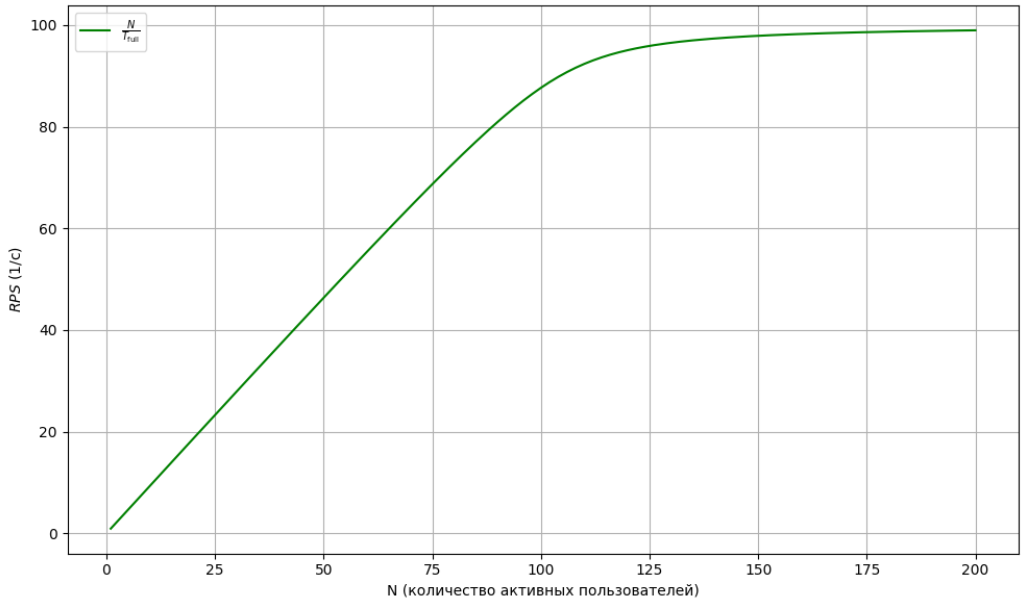
\includegraphics[width=1\textwidth]{../images/rps-from-n.png}
    \caption{Зависимость $RPS$ от $N$}
\end{figure}

При построении графика использованы следующие значения:

\begin{itemize}
    \item $T_{ping} = 60   \text{ мс}$
    \item $T_{wait} = 1000 \text{ мс}$
    \item $T_{handle} = 10 \text{ мс}$
\end{itemize}

Итак мы получили формулу, связывающую $RPS$ и степень сжатия. Перебором можно найти максимальный $RPS$. В этом заключается смысл алгоритма переключателя.

\subsection{Реализация переключателя}

Чтобы реализовать переключатель степени сжатия, используя указанный стек технологий, можно использовать один из 3-х способов:

\subsubsection{Дополнительный обратный прокси сервер на Express.js}

При первой попытке создания переключателя стало понятно, что стандартная реализация библиотеки Gzip и в целом Nginx не поддерживают динамическое изменение степени сжатия для конкретного HTTP запроса. То есть в Nginx можно прописать разное сжатие по адресам, это выглядит примерно так:

\begin{lstlisting}[
    basicstyle=\ttfamily\small,
    keywordstyle=\color{blue},
    commentstyle=\color{black},
    stringstyle=\color{red},
    numbers=left,
    numberstyle=\tiny\color{gray},
    frame=single,
    breaklines=true,
    backgroundcolor=\color{white}
]
http {
    gzip on;
    gzip_types application/json text/plain text/css application/javascript application/xml;
    gzip_min_length 100;
    gzip_vary on;
    include /etc/nginx/conf.d/*.conf;

    server {
        listen 3002;
        add_header Vary Accept-Encoding;

        location ^~ /gzip/1/ {
            gzip_comp_level 1;
            rewrite ^/gzip/1/(.*)$ /$1 break;
            proxy_pass http://server:3001;
        }

        location ^~ /gzip/2/ {
            gzip_comp_level 2;
            rewrite ^/gzip/2/(.*)$ /$1 break;
            proxy_pass http://server:3001;
        }
    }
}
\end{lstlisting}

То есть для адреса `/gzip/1/*` применяем сжатие gzip 1, для адреса `/gzip/2/*` применем сжатие gzip 2 и т.д. Но браузер сам не будет получать информацию о загрузке сети и процессора сервера и перенаправлять запросы. Для этой задачи я использовал ещё один обратный прокси сервер на Express js, который проверял с заданным промежутком загрузку процессора и перенаправлял запрос `/someadress/` на `/gzip/n/someadress`.

К сожалению, затраты на создание ещё одного прокси оказались слишком велики, при любой конфигурации сети,
количество обработанных запросов такого переключателя было более чем на 10\% меньше чем статическое сжатие с помощью Nginx gzip 1.

\subsubsection{Реконфигуратор Nginx }

Существует команда `nginx -s reload`, которая выполняет безопасную перезагрузку конфигурационного файла

Получив сигнал, главный процесс проверяет правильность синтаксиса нового конфигурационного файла и пытается применить содержащуюся в нём конфигурацию:
\begin{itemize}
    \item Если это удаётся, главный процесс запускает новые рабочие процессы и отправляет сообщения старым рабочим процессам с требованием завершиться.
    \item В противном случае главный процесс откатывает изменения и продолжает работать со старой конфигурацией.
\end{itemize}

Старые рабочие процессы, получив команду завершиться, прекращают принимать новые запросы и продолжают обслуживать текущие запросы, пока все такие запросы не будут обслужены. После этого старые рабочие процессы завершаются.

Таким образом, эта команда позволяет в реальном времени без опасения потерять необработанные запросы сменить конфигурационный файл. Было создано 10 конфигурационных файлов: 1 без сжатия, 9 - для каждого уровня gzip. И с помощью дополнительной
программы менял их и перезагружал Nginx

\subsubsection{Модуль для Nginx}

Для Nginx можно написать свой модуль, который будет выполнять роль переключателя. В ходе данной работы я его не реализовал

\section{Общие выводы}

В ходе работы мы рассмотрели применение методов сжатия на примере реального веб-приложения для оптимизации таких ключевых метрик, как LCP и RPS.
Проведён сравнительный анализ с точки зрения степени сжатия, времени компрессии/декопрессии. Построена модель backend сервера,
найдены зависимости между нагрузкой на сеть и на ЦП. Построена модель для оценки времени запроса от сервера.
Были получены условия на выбор оптимальных параметров сжатия и на их основе даны практические рекомендации.
Реализовано и предложено несколько вариантов переключателя, используя уже существующий стек технологий.

Стоит отметить, что в случае моего сервера, переключатель не потребовался. Вне зависимости от числа пользователей,
накладные расходы на сжатие полностью окупились бенефитами от снижения нагрузки на сеть.

\subsection{План дальнейших исследований}

Хотелось бы провести замеры на крупном проекте с высоким трафиком. Применить теорию массового обслуживания для установления более точных
соотношений между метриками. Реализовать модуль для Nginx, чтобы снизить накладные расходы на переключатель.

\begin{thebibliography}{9}
    \bibitem{rfc1950}
    P. Deutsch, J. Gailly,
    \textit{RFC 1950: ZLIB Compressed Data Format Specification},
    IETF, May 1996.
    \url{https://tools.ietf.org/html/rfc1950}

    \bibitem{rfc1951}
    P. Deutsch,
    \textit{RFC 1951: DEFLATE Compressed Data Format Specification},
    IETF, May 1996.
    \url{https://tools.ietf.org/html/rfc1951}

    \bibitem{rfc1952}
    P. Deutsch,
    \textit{RFC 1952: GZIP File Format Specification},
    IETF, May 1996.
    \url{https://tools.ietf.org/html/rfc1952}

    \bibitem{brotli}
    L. Zhelyazkov et al.,
    \textit{RFC 7932: Brotli Compressed Data Format},
    IETF, July 2016.
    \url{https://tools.ietf.org/html/rfc7932}

    \bibitem{rfc2616}
    R. Fielding et al.,
    \textit{RFC 2616: Hypertext Transfer Protocol -- HTTP/1.1},
    IETF, June 1999 (Section 3.5: Content Codings).
    \url{https://tools.ietf.org/html/rfc2616#section-3.5}

    \bibitem{compression-book}
    Ватолин Д., Ратушняк А., Смирнов М., Юкин В.,
    \textit{Методы сжатия данных. Устройство архиваторов, сжатие изображений и видео},
    М.: ДИАЛОГ-МИФИ, 2002, с. 75--116.

    \bibitem{data-compression}
    D. Salomon, G. Motta,
    \textit{Handbook of Data Compression},
    5th ed., Springer, 2010.

    \bibitem{express}
    Express.js Documentation,
    \textit{Express - Node.js web application framework},
    \url{https://expressjs.com/}

    \bibitem{react}
    React Documentation,
    \textit{React - A JavaScript library for building user interfaces},
    \url{https://reactjs.org/docs/getting-started.html}

    \bibitem{node}
    Node.js Documentation,
    \textit{Node.js JavaScript Runtime},
    \url{https://nodejs.org/en/docs/}

    \bibitem{k6}
    k6 Documentation,
    \textit{k6 - Open-source load testing tool},
    \url{https://k6.io/docs/}

    \bibitem{nginx}
    NGINX Documentation,
    \textit{NGINX - High Performance Load Balancer, Web Server \& Reverse Proxy},
    \url{https://nginx.org/en/docs/}

    \bibitem{compression-algorithms}
    M. Nelson, J. Gailly,
    \textit{The Data Compression Book},
    2nd ed., M\&T Books, 1995.

    \bibitem{modern-compression}
    I.H. Witten et al.,
    \textit{Managing Gigabytes: Compressing and Indexing Documents and Images},
    Morgan Kaufmann, 1999.
\end{thebibliography}
\end{document}